
%%%%%%%%%%%%%%%%%%%% 基本概念 %%%%%%%%%%%%%%%%%%%%%

\chapter{基本概念}\label{chap:BasicNotion}

\section{向量空间}\label{sec:vector_space}

向量空间$V$是一系列对象所构成的（非空）集合，这些对象称为向量（本书中以粗体小写字母表示，例如$\mathbf{v}$）。其上还定义了两种运算——向量的加法以及向量与数（标量）的乘法\footnote{我们需要让向量和其他对象看起来有些区别，因此在本书中我们使用粗体小写字母来表示向量，并用正体小写字母来表示数（标量）。一些（进阶的）教材中，拉丁字母用于表示向量而希腊字母用于表示标量；更为进阶的教材里，任意字母可用于表示任意对象，而读者须从上下文推断每个符号的含义。我认为，尤其对于初学者而言，对不同对象加以视觉上的区分是有助于理解的，因此总用粗体小写字母来表示向量。在黑板上，则用箭头来标识向量（如$\vec{v}$所示）。}，这两种运算满足所得结果总属于$V$，以及以下的八条性质（所谓向量空间的{\bf 公理}）：

前 4 条性质是关于加法的：\marginpar{\small 问题来了：“这些性质怎么记得住呢？”回答是，并不需要记忆，详见后文！}
\begin{enumerate}
    \item 交换律：对于所有 $\mathbf{v},\mathbf{w}\in V$，都有$\mathbf{v} + \mathbf{w} = \mathbf{w} + \mathbf{v}$；
    \item 结合律：对于所有 $\mathbf{u},\mathbf{v},\mathbf{w}\in V$，都有$(\mathbf{u}+\mathbf{v})+\mathbf{w}=\mathbf{u}+(\mathbf{v}+\mathbf{w})$；
    \item 零向量：存在一个特殊的向量，记作$\mathbf{0}$，其满足$\mathbf{v}+\mathbf{0} = \mathbf{v}$对于所有$\mathbf{v}\in V$都成立；
    \item 加法逆元：对于每个向量$\mathbf{v}\in V$，都存在向量$\mathbf{w}\in V$使得$\mathbf{v}+\mathbf{w}=\mathbf{0}$。这一加法逆元常记作$-\mathbf{v}$；
\end{enumerate}

接下来两条性质是有关乘法的：

\begin{enumerate}[start=5]
    \item 乘法恒等元：对于所有$\mathbf{v}\in V$，都有$1\mathbf{v}=\mathbf{v}$；
    \item 乘法结合律：对于所有$\mathbf{v}\in V$和所有标量$\alpha,\beta$，都有$(\alpha\beta)\mathbf{v} = \alpha(\beta\mathbf{v})$；
\end{enumerate}

最后是两条分配性质，它们将乘法与加法联系起来：

\begin{enumerate}[start=7]
    \item 对于所有$\mathbf{u},\mathbf{v}\in V$和所有标量$\alpha$，都有$\alpha(\mathbf{u}+\mathbf{v})=\alpha\mathbf{u}+\alpha\mathbf{v}$；
    \item 对于所有$\mathbf{v}\in V$和所有标量$\alpha,\beta$，都有$(\alpha+\beta)\mathbf{v}=\alpha\mathbf{v}+\beta\mathbf{v}$。
\end{enumerate}

\begin{remark*}
    上述性质看起来很难记忆，但其实没必要记——它们就是标量代数的运算律，而这些内容你在中学期间就已经知道了。唯一新出现的难点是，你需要理解运算可作用的对象。你可以将向量相加，也可以将向量与数（标量）相乘。当然，你还可以对于数进行之前你学过的所有运算。然而，你不能将两个向量相乘，或将向量和数加在一起。
\end{remark*}

\begin{remark*}
    容易证明，零向量$\mathbf{0}$是唯一的，并且对于给定$\mathbf{v}\in V$，其加法逆元$-\mathbf{v}$也是唯一的。

    同样，（利用性质5、6和8）不难证明$\mathbf{0} = 0\mathbf{v}$对所有$\mathbf{v}\in V$都成立，且有$-\mathbf{v}=(-1)\mathbf{v}$。注意，在证明过程中，我们还需用到向量空间的其他性质，特别是性质3和4。
\end{remark*}

若标量为实数，那么我们称$V$为{\bf 实}向量空间。若标量为复数，意即我们可将向量与复数相乘，那么我们称$V$为{\bf 复}向量空间。

注意，任何的复向量空间也是实向量空间（如果我们可以做复数乘法，那么也可以做实数乘法），但反之不成立。

还可以考虑标量为任意的域$\mathbb{F}$中的元素的情况。\marginpar{\small 如果你不知道什么是域也不必担心，因为在这本书中我们只考虑实向量空间和复向量空间。}在这种情况里，我们说$V$是域$\mathbb{F}$上的向量空间。尽管本书的许多章节（特别地，第 \ref{chap:BasicNotion} 至 \ref{chap:Determinant} 章的全部内容）对于一般的域都适用，在本书中我们只考虑实向量空间和复向量空间。

如果我们不指明标量集合或使用$\mathbb{F}$来指代之，那么有关结论就对实向量空间和复向量空间都成立。如果需要区分实向量空间和复向量空间，那么我们就会说清楚到底在考虑何种情况。

注意，在“任意的域上的向量空间”这一定义中，我们{\bf 要求}标量集合为域，这样我们总是可以与非零标量做除法（并且不产生余数）。于是，向量空间的标量集可以取为有理数集，但不能取为整数集。

\subsection{例子}
\begin{example*}
    向量空间$\mathbb{R}^n$由长度为$n$的列向量（如下）所构成：
    \[\mathbf{v}=\begin{pmatrix}v_1\\v_2\\\vdots\\v_n\end{pmatrix}\]
    其中各项为实数。加法和乘法是逐项定义的，也即
    \[\alpha\begin{pmatrix}v_1\\v_2\\\vdots\\v_n\end{pmatrix}=\begin{pmatrix}\alpha v_1\\\alpha v_2\\\vdots\\\alpha v_n\end{pmatrix},\quad\begin{pmatrix}v_1\\v_2\\\vdots\\v_n\end{pmatrix}+\begin{pmatrix}w_1\\w_2\\\vdots\\w_n\end{pmatrix}=\begin{pmatrix}v_1+w_1\\v_2+w_2\\\vdots\\v_n+w_n\end{pmatrix}\]
\end{example*}

\begin{example*}
    向量空间$\mathbb{C}^n$同样由长度为$n$的列向量所构成，只是向量中各项为复数。加法和乘法与$\mathbb{R}^n$中的定义相同，唯一的区别在于如今可以将向量与{\bf 复}数相乘，也即，$\mathbb{C}^n$为{\bf 复}向量空间。
\end{example*}

本书中许多结论对于$\mathbb{R}^n$和$\mathbb{C}^n$都成立，在这样的情况下，我们将使用$\mathbb{F}^n$这个记号。

\begin{example*}
    向量空间$M_{m\times n}$（也记作$M_{m,n}$）由$m\times n$矩阵构成，加法和标量乘法是逐项定义的。如果我们限制各项为实数（并且只允许与实数相乘），那么我们就得到了一个实向量空间；如果我们允许各项为复数（并且允许与复数相乘），那么我们就得到了一个复向量空间。

    正式而言，我们需要区分实数与复数情形，也即分别写为$M_{m, n}^{\mathbb{R}}$和$M_{m, n}^{\mathbb{C}}$。然而，在大多数场合中，实数和复数情形并没有区别，于是也没有必要明确到底在考虑哪种情形。如果有所区别，我们会说清楚考虑的是哪种情况。
\end{example*}

\begin{remark*}
    如上所提到的，向量空间的公理仅仅是实数或复数的通常代数运算规则，因此如果我们将标量（数）视作向量，那么所有的公理都是成立的。于是，实数集合$\mathbb{R}$是实向量空间，复数集合$\mathbb{C}$是复向量空间。

    更重要的是，由于在上面的例子中，所有的向量运算（加法和标量乘法）都是逐项进行的，因此在这些例子中向量空间的公理是自动满足的，因为这些公理对标量成立（你能看出原因吗？）。因此，无需检验这些公理，我们就能得知上述例子中的集合的确是向量空间！

    同样的道理也适用于下面的例子，此处多项式的系数充当了（上述列向量或矩阵中）各项的角色。
\end{remark*}

\begin{example*}
    由次数至多为$n$的多项式所构成的向量空间$\mathbb{P}_n$，其中各元素$p$都是多项式，形式如下：\[p(t) = a_0 + a_1t + a_2t^2 + \dots +a_nt^n,\]
    其中$t$为自变量。注意，有些（甚至全部）系数$a_k$可以取$0$。

    系数$a_k$为实数时，我们就得到了一个实向量空间；系数$a_k$为复数时，此空间则为复向量空间。同样，仅在有必要的时候我们才说明考虑的是实数情形还是复数情形，否则所讨论的内容在两种情况下都适用。
\end{example*}

{\bf 问题：}上面这几个例子中的零向量是什么？

\subsection{矩阵记号}\label{subsec:matrix_notation}

一个$m\times n$的矩阵是一个有$m$行$n$列的数阵。这个阵列中的元素称为矩阵的{\bf 项}。

将矩阵的项记作带下标的字母是很方便的：第一个下标代表该项的行号，而第二个下标则代表列号。例如
\begin{equation}\label{matrix_notation}
    A=(a_{j,k})_{j=1,k=1}^{m,\quad n}=\begin{pmatrix}a_{1,1}&a_{1,2}&\ldots&a_{1,n}\\a_{2,1}&a_{2,2}&\ldots&a_{2,n}\\\vdots&\vdots&&\vdots\\a_{m,1}&a_{m,2}&\ldots&a_{m,n}\end{pmatrix}
\end{equation}
就是$m\times n$矩阵的通常表示形式。

矩阵$A$中的第$j$行第$k$列的项往往表示为$A_{j,k}$或$(A)_{j,k}$，有时也像上面的式 \eqref{matrix_notation} 那样用小写字母加下标来表示。

给定一矩阵$A$，其{\bf 转置}（或转置矩阵）$A^T$定义为将$A$的行变为列所得的矩阵。例如
\[\begin{pmatrix}1&2&3\\4&5&6\end{pmatrix}^T=\begin{pmatrix}1&4\\2&5\\3&6\end{pmatrix}.\]
因此，$A^T$的各列就是$A$的各行。反之亦然：$A^T$的各行就是$A$的各列。

正式的定义是：$(A^T)_{j,k}=(A)_{k,j}$，意为：$A^T$的第$j$行第$k$列的项等于$A$的第$k$行第$j$列的项。

就线性变换而言，矩阵的转置可用于给出一个很优美的阐释，也即其能导出所谓{\bf 伴随}变换，我们将在后面详细研究它，目前转置仅仅是一种有用且正式的运算。

转置的用处首先在于使我们得以将列向量$\mathbf{x}\in\mathbb{F}^n$（回想一下，$\mathbb{F}$是指$\mathbb{R}$或$\mathbb{C}$）写为$\mathbf{x} = (x_1,x_2,\dots,x_n)^T$。如果我们将列向量竖着写，那么其占据的空间就会大大增加。

\begin{problemset}
\item 令$\mathbf{x}=(1,2,3)^{T},\mathbf{y}=(y_{1},y_{2},y_{3})^{T},\mathbf{z}=(4,2,1)^{T}$。计算$2\mathbf{x},3\mathbf{y},\mathbf{x}+2\mathbf{y}-3\mathbf{z}$。
\item 下面哪些集合（具有自然的加法和标量乘法运算）是向量空间？论证你的结论。
\begin{probenumerate}
    \item 所有区间$[0,1]$上的连续函数所成的集合；
    \item 所有区间$[0,1]$上的非负函数所成的集合；
    \item 所有次数{\bf 恰}为$n$的多项式所成的集合；
    \item 所有$n\times n$对称矩阵所成的集合，即所有满足$A^T=A$的矩阵$A=\{a_{j,k}\}_{j,k=1}^n$所成的集合。
\end{probenumerate}
\item 判断正误：
\begin{probenumerate}
    \item 每个向量空间都包含零向量；
    \item 一向量空间可包含多个零向量；
    \item $m\times n$矩阵有$m$行$n$列；
    \item 若$f$和$g$是次数为$n$的多项式，那么$f+g$也是次数为$n$的多项式；
    \item 若$f$和$g$是次数至多为$n$的多项式，那么$f+g$也是次数至多为$n$的多项式。
\end{probenumerate}
\item 证明：向量空间$V$的零向量$\mathbf{0}$唯一。
\item 向量空间$M_{2\times 3}$的零向量是何矩阵？
\item 证明：向量空间公理4所定义的加法逆元是唯一的。
\item 证明：$0\mathbf{v} = \mathbf{0}$对于所有向量$\mathbf{v}\in V$都成立。
\item 证明：对于所有向量$\mathbf{v}$，其加法逆元$-\mathbf{v}$由$(-1)\mathbf{v}$给出。
\end{problemset}

\section{线性组合、基}

令$V$为一向量空间，并令$\mathbf{v}_{1},\mathbf{v}_{2},\ldots,\mathbf{v}_{p}\in V$为一系列向量。向量$\mathbf{v}_{1},\mathbf{v}_{2},\ldots,\mathbf{v}_{p}$的{\bf 线性组合}是形式如下的求和式：
\[\alpha_1\mathbf{v}_1+\alpha_2\mathbf{v}_2+\ldots+\alpha_p\mathbf{v}_p=\sum_{k=1}^p\alpha_k\mathbf{v}_k.\]

\begin{definition}
    称一组向量\footnote{原书对于若干向量有两种表达：“a system of vectors”和“a set of vectors”，此处一律采用国内通行翻译“向量组”。——译者注}$\mathbf{v}_{1},\mathbf{v}_{2},\ldots,\mathbf{v}_{n}\in V$为（向量空间$V$的）基，若任意向量$\mathbf{v}\in V$都能被{\bf 唯一}写成线性组合的形式：\[\mathbf{v}=\alpha_1\mathbf{v}_1+\alpha_2\mathbf{v}_2+\ldots+\alpha_n\mathbf{v}_n=\sum_{k=1}^n\alpha_k\mathbf{v}_k.\]
    系数$\alpha_1,\alpha_2,\dots,\alpha_n$称为向量$\mathbf{v}$（在基下，或者说关于基$\mathbf{v}_{1},\mathbf{v}_{2},\ldots,\mathbf{v}_{n}$）的{\bf 坐标}。

    $\mathbf{v}_{1},\mathbf{v}_{2},\ldots,\mathbf{v}_{n}$是基的另一种表述是，方程$x_{1}\mathbf{v}_{1}+x_{2}\mathbf{v}_{2}+\ldots+x_{n}\mathbf{v}_{n}=\mathbf{v}$（未知数为各$x_k$）对于任意右端项$\mathbf{v}$皆有唯一解。
\end{definition}

在讨论基的性质之前，首先给出一些例子来说明“基”这种对象确实存在，并且研究它们是有意义的。

\begin{example}
    在这第一个例子当中，向量空间$V$等于$\mathbb{F}^n$，其中$\mathbb{F}$是$\mathbb{R}$或$\mathbb{C}$。考虑向量
    \[\mathbf{e}_1=\begin{pmatrix}1\\0\\0\\\vdots\\0\end{pmatrix},\quad\mathbf{e}_2=\begin{pmatrix}0\\1\\0\\\vdots\\0\end{pmatrix},\quad\mathbf{e}_3=\begin{pmatrix}0\\0\\1\\\vdots\\0\end{pmatrix},\ldots,\quad\mathbf{e}_n=\begin{pmatrix}0\\0\\0\\\vdots\\1\end{pmatrix},\]
    （向量$\mathbf{e}_k$除第$k$项为$1$外，其余各项均为$0$）。
    
    向量组$\mathbf{e}_1,\mathbf{e}_2,\dots,\mathbf{e}_n$是$\mathbb{F}^n$的基。的确，任意向量\[\mathbf{v}=\begin{pmatrix}x_1\\x_2\\\vdots\\x_n\end{pmatrix}\in\mathbb{F}^n\]
    都能被表示成线性组合
    \[\mathbf{v}=x_1\mathbf{e}_1+x_2\mathbf{e}_2+\ldots +x_n\mathbf{e}_n=\sum_{k=1}^nx_k\mathbf{e}_k\]
    且该表示唯一。向量组$\mathbf{e}_1,\mathbf{e}_2,\dots,\mathbf{e}_n$称为$\mathbb{F}^n$的{\bf 标准基}。
\end{example}

\begin{example}
    本例中考虑的是次数至多为$n$的多项式所构成的向量空间$\mathbb{P}_n$。考虑定义如下的向量（多项式）$\mathbf{e}_0,\mathbf{e}_1,\mathbf{e}_2,\dots,\mathbf{e}_n\in \mathbb{P}_n$
    \[\mathbf{e}_0:=1,\quad\mathbf{e}_1:=t,\quad\mathbf{e}_2:=t^2,\quad\mathbf{e}_3:=t^3,\quad\ldots,\quad\mathbf{e}_n:=t^n.\]
    显然，对任意多项式$p$，$p(t)=a_0+a_1t+a_2t^2+\ldots+a_nt^n$，其均能被唯一表示为
    \[p=a_0\mathbf{e}_0+a_1\mathbf{e}_1+\ldots+a_n\mathbf{e}_n.\]
    因此向量组$\mathbf{e}_0,\mathbf{e}_1,\mathbf{e}_2,\ldots,\mathbf{e}_n\in\mathbb{P}_n$是$\mathbb{P}_n$的基。我们称其为$\mathbb{P}_n$的标准基。
\end{example}

\begin{remark}\label{remark:fn_to_abstract}
    若向量空间$V$有基$\mathbf{v}_{1},\mathbf{v}_{2},\ldots,\mathbf{v}_{n}$，\marginpar{\small 这个注记很重要，整本书都会用到它。它使我们得以将适用于标准向量空间$\mathbb{F}^n$的各种表述迁移至具有基$\mathbf{v}_{1},\mathbf{v}_{2},\ldots,\mathbf{v}_{n}$的向量空间$V$。}那么任意向量$\mathbf{v}$都能被线性组合式$\mathbf{v}=\sum_{k=1}^{n}\alpha_{k}\mathbf{v}_{k}$中的系数唯一决定。因此，如果我们将各系数$\alpha_k$写在一列中，那么我们处理任意向量就如同处理列向量一样，也就是如同处理$\mathbb{F}^n$中的元素一样（此处$\mathbb{F}$仍然代表$\mathbb{R}$或$\mathbb{C}$，不过此处的结论对于任意的域$\mathbb{F}$也是成立的）。

    这就是说，若$\mathbf{v}=\sum_{k=1}^{n}\alpha_{k}\mathbf{v}_{k}$且$\mathbf{w}=\sum_{k=1}^{n}\beta_{k}\mathbf{v}_{k}$，则
    \[\mathbf{v}+\mathbf{w}=\sum_{k=1}^n\alpha_k\mathbf{v}_k+\sum_{k=1}^n\beta_k\mathbf{v}_k=\sum_{k=1}^n(\alpha_k+\beta_k)\mathbf{v}_k,\]
    即为了得到求和结果的坐标所构成的列向量，只需将各求和项的坐标所构成的列向量相加。类似地，为了得到$\alpha\mathbf{v}$的坐标，我们只需将$\mathbf{v}$的坐标所构成的列向量乘以$\alpha$。
\end{remark}

\subsection{生成组与线性无关组}

基的定义中说到，任意向量都能被唯一表示成基向量的线性组合。这个说法其实包含两方面：一是表达式存在，二是表达式唯一。让我们分开来分析这两个方面。

如果我们只考虑存在性，我们就得到下面的概念：

\begin{definition}
    称一组向量$\mathbf{v}_{1},\mathbf{v}_{2},\ldots,\mathbf{v}_{p}\in V$为$V$中的生成组（也称为{\bf 张成组}或{\bf 完备组}），若任意向量$\mathbf{v}\in V$都能被写成线性组合的形式：\[\mathbf{v}=\alpha_1\mathbf{v}_1+\alpha_2\mathbf{v}_2+\ldots+\alpha_p\mathbf{v}_p=\sum_{k=1}^p\alpha_k\mathbf{v}_k.\]
\end{definition}

该定义与基的定义的唯一区别在于，我们并不假设上述表示形式唯一。

此处{\bf 生成}、{\bf 张成}和{\bf 完备}是同义词。我本人更喜欢“完备”这个词，这是由于我在算子理论方面的专业背景。“生成”和“张成”则更经常用于线性代数教材中。

显然，任一基都是张成（完备）向量组。并且，如果我们向基$\mathbf{v}_{1},$ $\mathbf{v}_{2},\ldots,\mathbf{v}_{n}$中加入若干向量$\mathbf{v}_{n+1},\ldots,\mathbf{v}_{p}$，那么新的向量组是张成（完备）向量组。的确如此：我们可以将任意向量表示成$\mathbf{v}_{1},\mathbf{v}_{2},\ldots,$ $\mathbf{v}_{n}$的线性组合，并直接忽略新加入的向量（取对应的系数$\alpha_k=0$）。

现在，让我们将注意力转向唯一性。我们不想产生存在性方面的顾虑，因此我们考虑零向量$\mathbf{0}$，其总是能够以线性组合式表出。

\begin{definition*}
    称线性组合$\alpha_{1}\mathbf{v}_{1}+\alpha_{2}\mathbf{v}_{2}+\ldots+\alpha_{p}\mathbf{v}_{p}$是{\bf 平凡的}，若$\alpha_k = 0\ \forall k$。
\end{definition*}

平凡的线性组合总等于$\mathbf{0}$（无论向量$\mathbf{v}_1,\mathbf{v}_2,\ldots,\mathbf{v}_p$是什么），这可能也是其名称的来历。

\begin{definition*}
    称一组向量$\mathbf{v}_{1},\mathbf{v}_{2},\ldots,\mathbf{v}_{p}\in V$为{\bf 线性无关的}，若$\mathbf{v}_{1},\mathbf{v}_{2},\ldots,\mathbf{v}_{p}$只有平凡线性组合（$\sum_{k=1}^{p}\alpha_{k}\mathbf{v}_{k}$，其中$\alpha_{k}=0\ \forall k$）等于$\mathbf{0}$。

    换言之，向量组$\mathbf{v}_{1},\mathbf{v}_{2},\ldots,\mathbf{v}_{p}$是线性无关的，当且仅当方程$x_1\mathbf{v}_1+x_2\mathbf{v}_2+\ldots+x_p\mathbf{v}_p=\mathbf{0}$（未知数为$x_k$）仅有平凡解（$x_{1}=x_{2}=\ldots=x_{p}=0$）。
\end{definition*}

若一向量组不是线性无关的，就称其为{\bf 线性相关的}。通过取线性无关定义的否定，我们得到以下定义：

\begin{definition*}
    称一组向量$\mathbf{v}_{1},\mathbf{v}_{2},\ldots,\mathbf{v}_{p}\in V$为{\bf 线性相关的}，若$\mathbf{0}$可被表示为非平凡的线性组合$\mathbf{0}=\sum_{k=1}^{p}\alpha_{k}\mathbf{v}_{k}$。此处的“非平凡”是指至少一个系数$\alpha_{k}$是非零的。这可以写为（也通常表示为）$\sum_{k=1}^{p}|\alpha_{k}|\neq0$。
\end{definition*}

换种方式表述该定义，我们可以说，向量组$\mathbf{v}_{1},\mathbf{v}_{2},\ldots,\mathbf{v}_{p}$是线性相关的，当且仅当存在标量$\alpha_1,\alpha_2,\ldots,\alpha_p$且$\sum_{k=1}^{p}|\alpha_{k}|\neq0$使得\[\sum_{k=1}^p\alpha_k\mathbf{v}_k=\mathbf{0}.\]

还有一种定义（以方程的语言表述）是：向量组$\mathbf{v}_{1},\mathbf{v}_{2},\ldots,\mathbf{v}_{p}$是线性相关的，当且仅当方程\[x_1\mathbf{v}_1+x_2\mathbf{v}_2+\ldots+x_p\mathbf{v}_p=\mathbf{0}\]
（未知数为$x_k$）有非平凡解。此处的“非平凡”还是指至少一个$x_{k}$是非零的，并可写作$\sum_{k=1}^{p}|x_{k}|\neq0$。

以下命题又给出了线性相关组的一种描述。
\begin{proposition}
    一组向量$\mathbf{v}_{1},\mathbf{v}_{2},\ldots,\mathbf{v}_{p}\in V$是线性相关的，当且仅当其中有一向量$\mathbf{v}_{k}$可被表示成其他向量的线性组合
    \begin{equation}\label{eq_2_1}
        \mathbf{v}_k=\sum_{\begin{subarray}{c}j=1\\j\neq k\end{subarray}}^p\beta_j\mathbf{v}_j.
    \end{equation}
\end{proposition}
\begin{proof}
    假设向量组$\mathbf{v}_{1},\mathbf{v}_{2},\ldots,\mathbf{v}_{p}$是线性相关的。那么存在标量$\alpha_{k}$，\\$\sum_{k=1}^{p}|\alpha_{k}|\neq0$使得
    \[\alpha_1\mathbf{v}_1+\alpha_2\mathbf{v}_2+\cdots+\alpha_p\mathbf{v}_p=\mathbf{0}.\]
    令$k$为使得$\alpha_k\ne 0$的下标。于是，将除了$\alpha_{k}\mathbf{v}_{k}$之外的项移到右端可得\[\alpha_k\mathbf{v}_k=-\sum_{\begin{subarray}{c}j=1\\j\neq k\end{subarray}}^p\alpha_j\mathbf{v}_j.\]
    将两边都除以$\alpha_k$可得式 \eqref{eq_2_1}，其中$\beta_j = -\alpha_j/\alpha_k$。

    另一方面，若 \eqref{eq_2_1} 成立，那么$\mathbf{0}$可被表示为非平凡线性组合\[\mathbf{v}_k-\sum_{\begin{subarray}{c}j=1\\j\neq k\end{subarray}}^p\beta_j\mathbf{v}_j=\mathbf{0}.\]
\end{proof}

显然，任一基都是线性无关组。的确如此：若向量组$\mathbf{v}_{1},\mathbf{v}_{2},\ldots,\mathbf{v}_{n}$是基，那么$\mathbf{0}$可被唯一表示为\[\mathbf{0}=\alpha_1\mathbf{v}_1+\alpha_2\mathbf{v}_2+\cdots+\alpha_n\mathbf{v}_n=\sum_{k=1}^n\alpha_k\mathbf{v}_k.\]
由于$\mathbf{0}$总可被平凡线性组合表出，所以平凡线性组合就是{\bf 唯一}线性表出$\mathbf{0}$的方法。

\marginpar{\small 在许多教材中，基被定义为既完备又线性无关的向量组。由命题 \ref{prop:complete_li_basis}，这种定义和本书的定义是等价的。}

所以，如我们已经讨论的，若一向量组是基，则其是完备（生成）组，也是线性无关组。下面命题表明，这句话反过来也是成立的。

\begin{proposition}\label{prop:complete_li_basis}
    向量组$\mathbf{v}_{1},\mathbf{v}_{2},\ldots,\mathbf{v}_{n}\in V$是基，当且仅当其既是完备（生成）组又线性无关。
\end{proposition}

\begin{proof}
    我们已经知道基一定是既完备又线性无关的，所以该命题的一个方向已经得证了。

    让我们证明另一个方向。设向量组$\mathbf{v}_{1},\mathbf{v}_{2},\ldots,\mathbf{v}_{n}$是线性无关且完备的。取任意向量$\mathbf{v}\in V$。因为向量组$\mathbf{v}_{1},\mathbf{v}_{2},\ldots,\mathbf{v}_{n}$是完备（生成）组，因此$\mathbf{v}$可表示为\[\mathbf{v}=\alpha_1\mathbf{v}_1+\alpha_2\mathbf{v}_2+\cdots+\alpha_n\mathbf{v}_n=\sum_{k=1}^n\alpha_k\mathbf{v}_k.\]
    我们只需证明此表达式是唯一的。

    设$\mathbf{v}$还可被表示为\[\mathbf{v}=\sum_{k=1}^{n}\widetilde{\alpha}_{k}\mathbf{v}_{k}.\]
    那么\[\sum_{k=1}^n(\alpha_k-\widetilde{\alpha}_k)\mathbf{v}_k=\sum_{k=1}^n\alpha_k\mathbf{v}_k-\sum_{k=1}^n\widetilde{\alpha}_k\mathbf{v}_k=\mathbf{v}-\mathbf{v}=\mathbf{0}.\]
    因为该组是线性无关的，所以$\alpha_k-\widetilde{\alpha}_k = 0\ \forall k$，从而表达式$\mathbf{v}=\alpha_{1}\mathbf{v}_{1}+\alpha_{2}\mathbf{v}_{2}+\ldots+\alpha_{n}\mathbf{v}_{n}$唯一。
\end{proof}

\begin{remark*}
    在许多教材中，基被定义为既完备又线性无关的向量组（由命题 \ref{prop:complete_li_basis}，这种定义和本书的定义是等价的）。尽管这种定义比本书所示的定义更为常见，我还是更喜欢后者。它强调了基的主要性质，即任意向量都能被基向量的线性组合唯一表出。
\end{remark*}

\begin{proposition}\label{prop:generating_contain_basis}
    任意（有限）生成组包含一个基。
\end{proposition}

\begin{proof}
    设$\mathbf{v}_{1},\mathbf{v}_{2},\ldots,\mathbf{v}_{p}\in V$是生成（完备）组。若它是线性无关的，它就是基，则我们已经达成目标。

    设它不是线性无关的，即它是线性相关的。那么存在向量$\mathbf{v}_k$，其可被表示为向量$\mathbf{v}_j,j\ne k$的线性组合。

    因为$\mathbf{v}_k$可被表示为向量$\mathbf{v}_j,j\ne k$的线性组合，向量组$\mathbf{v}_{1},\mathbf{v}_{2},\ldots,\mathbf{v}_{p}$的任意线性组合都可被除了$\mathbf{v}_{k}$之外的向量（即$\mathbf{v}_j,1\le j\le p, j\ne k$）的线性组合表示。因此，如果我们去除向量$\mathbf{v}_k$，新向量组将仍是完备的。

    若新向量组是线性无关的，那么我们达成了目标。若仍不是，则重复上述过程。

    在重复上述过程有限多次后，我们必得到一线性无关且完备的向量组，否则我们就会删除所有向量并且得到空组了。

    因此，任意有限的完备（生成）组都包含一完备的线性无关子集，也就是基。
\end{proof}

\begin{problemset}
    \item 求出$3\times 2$矩阵所成的向量空间$M_{3\times 2}$的基。
    \item 判断正误：
    \begin{probenumerate}
        \item 任意包含零向量的向量组都是线性相关的；
        \item 基必包含$\mathbf{0}$；
        \item 线性相关向量集合的子集是线性相关的；
        \item 线性无关向量集合的子集是线性无关的；
        \item 若$\alpha_{1}\mathbf{v}_{1}+\alpha_{2}\mathbf{v}_{2}+\ldots+\alpha_{n}\mathbf{v}_{n}=\mathbf{0}$，那么所有标量$\alpha_{k}$都为零。
    \end{probenumerate}
    \item 回想一下，称矩阵$A$是对称的，若$A^T=A$。写出由$2\times 2$对称矩阵所构成的向量空间的一个基（有很多可能的答案）。该基中包含几个元素？
    \item 写出由下列元素构成的空间的基：
    \begin{probenumerate}
        \item $3\times 3$对称矩阵；
        \item $n\times n$对称矩阵；
        \item $n\times n$反对称矩阵（$A^T=-A$）。
    \end{probenumerate}
    \item \label{ex:1_2_5}设向量组$\mathbf{v}_{1},\mathbf{v}_{2},\ldots,\mathbf{v}_{r}$是线性无关的，但不是生成组。证明：可以找到向量$\mathbf{v}_{r+1}$使得向量组$\mathbf{v}_{1},\mathbf{v}_{2},\ldots,\mathbf{v}_{r},\mathbf{v}_{r+1}$是线性无关的。{\bf 提示}：取$\mathbf{v}_{r+1}$为任一无法被表示为线性组合$\sum_{k=1}^r\alpha_k\mathbf{v}_k$的向量，再证明向量组$\mathbf{v}_{1},\mathbf{v}_{2},\ldots,\mathbf{v}_{r},\mathbf{v}_{r+1}$是线性无关的。
    \item 是否可能出现这样的情况：向量$\mathbf{v}_{1},\mathbf{v}_{2},\mathbf{v}_{3}$是线性相关的，但向量$\mathbf{w}_1=\mathbf{v}_1+\mathbf{v}_2,\mathbf{w}_2=\mathbf{v}_2+\mathbf{v}_3$与$\mathbf{w}_3=\mathbf{v}_3+\mathbf{v}_1$是线性{\bf 无关}的？
\end{problemset}

\section{线性变换、矩阵-向量乘法}

从集合$X$到集合$Y$的\textbf{变换}$T$是一种对应关系，\marginpar{\small “变换”、“映射”、\\“算子”、“函数”都是指同类对象。\footnotemark}将任意自变量（输入）$x\in X$对应到一值（输出）$y=T(x)\in Y$。\footnotetext{一般来说，算子的定义域和陪域一样。本书有些地方的“算子”实为一般的变换，翻译将予以区分。——译者注}

集合$X$称为$T$的{\bf 定义域}，集合$Y$称为$T$的{\bf 目标空间}或{\bf 陪域}。

我们记$T:X\to Y$表示$T$是定义域为$X$而目标空间为$Y$的变换。

\begin{definition}
    令$V,W$为（同一域$\mathbb{F}$上的）向量空间。称变换$T:V\to W$是线性的，若
    \begin{enumerate}
        \item $T(\mathbf{u}+\mathbf{v})=T(\mathbf{u})+T(\mathbf{v})\ \forall\mathbf{u},\mathbf{v}\in V$；
        \item $T(\alpha\mathbf{v})=\alpha T(\mathbf{v})$对所有$\mathbf{v}\in V$和所有标量$\alpha\in \mathbb{F}$都成立。
    \end{enumerate}
\end{definition}

性质1、2合起来等价于下面说法：
\begin{center}
    对于所有标量$\alpha,\beta$和所有$\mathbf{u},\mathbf{v}\in V$，有$T(\alpha\mathbf{u}+\beta\mathbf{v})=\alpha T(\mathbf{u})+\beta T(\mathbf{v})$。
\end{center}

\subsection{例子}

你之前已经和线性变换打过交道了——可能你还未曾意识到这一点。请看下面示出的例子。

\begin{example*}
    微分：令$V=\mathbb{P}_n$（次数至多为$n$的多项式所成的集合），$W=\mathbb{P}_{n-1}$，并令$T:\mathbb{P}_n\to \mathbb{P}_{n-1}$为微分算子
    \[T(p):=p^{\prime}\quad\forall p\in\mathbb{P}_n.\]
    因为$(f+g)^{\prime}=f^{\prime}+g^{\prime}$且$(\alpha f)^{\prime}=\alpha f^{\prime}$，所以这是一个线性变换。
\end{example*}

\begin{example*}
    旋转：在本例中$V=W=\mathbb{R}^2$（即通常的坐标平面），变换$T_{\gamma}:\mathbb{R}^2\to\mathbb{R}^2$将$\mathbb{R}^2$中的向量逆时针旋转$\gamma$弧度。因为$T_{\gamma}$是将平面整体做旋转，所以它会将用于定义两向量之和（平行四边形法则）的平行四边形整体做旋转（见图）。因此，其满足线性变换的性质1。容易看出，性质2也是成立的。
\end{example*}

\begin{figure}[htbp]
    \centering
    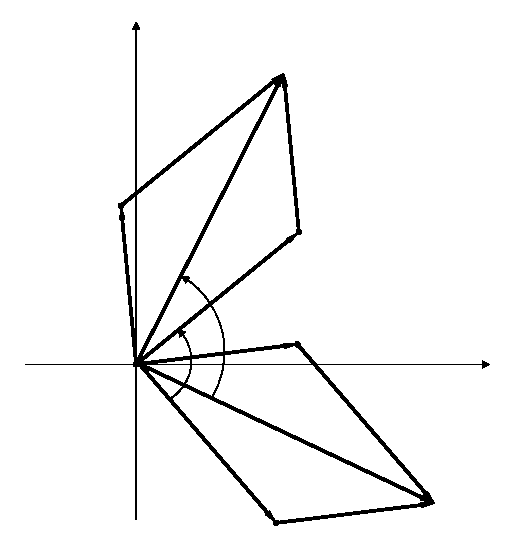
\includegraphics[scale=0.9]{figures/fig1_3_1.pdf}
    \caption{旋转}
\end{figure}

\begin{example*}
    反射：在本例中$V=W=\mathbb{R}^2$，变换$T_{\gamma}:\mathbb{R}^2\to\mathbb{R}^2$是关于第一轴的反射。可以从几何的角度证明该变换为线性的，但我们将用另一种方法来证明。

    方法是：写出$T$的表达式\[T\left(\begin{pmatrix}x_1\\x_2\end{pmatrix}\right)=\begin{pmatrix}x_1\\-x_2\end{pmatrix}\]
    根据该式，我们很容易检验该变换是线性的。
\end{example*}

\begin{example*}
    考察线性变换$T:\mathbb{R}\to\mathbb{R}$。任一此类变换都由下式给出\[T(x)=ax\quad\text{其中}~a=T(1).\]
    的确如此：\[T(x)=T(x\times1)=xT(1)=xa=ax.\]
    因此，$\mathbb{R}$上的任一线性变换仅仅是与常数的乘法。
\end{example*}

\subsection{\texorpdfstring{$\mathbb{F}^n\to \mathbb{F}^m$}{F**n到F**m}的线性变换、矩阵-列向量乘法}

线性变换$T:\mathbb{F}^n\to\mathbb{F}^m$也可用一乘法表示，不过不是与标量相乘，而是与矩阵相乘。

我们来看看是如何乘的。令$T:\mathbb{F}^n\to\mathbb{F}^m$为一线性变换。为了对所有向量$\mathbf{x}\in\mathbb{F}^{n}$计算$T(\mathbf{x})$，我们需要什么信息呢？我的观点是，知道$T$作用于$\mathbb{F}^{n}$中的标准基$\mathbf{e}_1,\mathbf{e}_2,\ldots,\mathbf{e}_n$的结果就足够了。也即，知道$\mathbb{F}^m$中的这$n$个向量（即若干长度为$m$的向量）就足够了：
\[\mathbf{a}_1=T(\mathbf{e}_1),\quad\mathbf{a}_2:=T(\mathbf{e}_2),\quad\ldots,\quad\mathbf{a}_n:=T(\mathbf{e}_n).\]
的确如此：令\[\mathbf{x}=\begin{pmatrix}x_1\\x_2\\\vdots\\x_n\end{pmatrix}.\]
那么$\mathbf{x}=x_{1}\mathbf{e}_{1}+x_{2}\mathbf{e}_{2}+\ldots+x_{n}\mathbf{e}_{n}=\sum_{k=1}^{n}x_{k}\mathbf{e}_{k}$，且有
\[T(\mathbf{x})=T\left(\sum_{k=1}^nx_k\mathbf{e}_k\right)=\sum_{k=1}^nT(x_k\mathbf{e}_k)=\sum_{k=1}^nx_kT(\mathbf{e}_k)=\sum_{k=1}^nx_k\mathbf{a}_k.\]

因此，如果我们将列向量$\mathbf{a}_{1},\mathbf{a}_{2},\ldots,\mathbf{a}_{n}$一起放入一矩阵$A=[\mathbf{a}_1,$ $\mathbf{a}_2,\ldots,\mathbf{a}_n]$（$\mathbf{a}_{k}$是$A$的第$k$列，$k=1,2,\ldots,n$），该矩阵就包含了$T$的所有信息。

下面我们说明如何定义矩阵和列向量的乘积才能将变换$T$表示为乘积$T(\mathbf{x})=A\mathbf{x}$。令
\[A=\begin{pmatrix}a_{1,1}&a_{1,2}&\ldots&a_{1,n}\\a_{2,1}&a_{2,2}&\ldots&a_{2,n}\\\vdots&\vdots&&\vdots\\a_{m,1}&a_{m,2}&\ldots&a_{m,n}\end{pmatrix}.\]

回想一下，$A$的第$k$列是向量$\mathbf{a}_{k}$，即\[\mathbf{a}_k=\begin{pmatrix}a_{1,k}\\a_{2,k}\\\vdots\\a_{m,k}\end{pmatrix}.\]
于是，如果我们要使$A\mathbf{x} = T(\mathbf{x})$，我们就有
\[A\mathbf{x}=\sum_{k=1}^nx_k\mathbf{a}_k=x_1\begin{pmatrix}a_{1,1}\\a_{2,1}\\\vdots\\a_{m,1}\end{pmatrix}+x_2\begin{pmatrix}a_{1,2}\\a_{2,2}\\\vdots\\a_{m,2}\end{pmatrix}+\ldots+x_n\begin{pmatrix}a_{1,n}\\a_{2,n}\\\vdots\\a_{m,n}\end{pmatrix}.\]

因此，矩阵-向量乘法应该按照下述“{\bf 列乘以坐标}”法则来进行：
\begin{center}
    \fbox{将矩阵的各列与向量的对应坐标相乘。}
\end{center}

\begin{example*}
    \[\begin{pmatrix}1&2&3\\3&2&1\end{pmatrix}\begin{pmatrix}1\\2\\3\end{pmatrix}=1\begin{pmatrix}1\\3\end{pmatrix}+2\begin{pmatrix}2\\2\end{pmatrix}+3\begin{pmatrix}3\\1\end{pmatrix}=\begin{pmatrix}14\\10\end{pmatrix}.\]
\end{example*}

“列乘以坐标”法则很适于并行计算，在之后的一些理论推导中也很重要。

不过，当手工进行计算时，逐项计算更为方便。这种计算可按以下“{\bf 行乘以列}”法则来进行：
\begin{center}
    \fbox{\parbox{0.8\linewidth}{要得到结果的第$k$项，我们需要将矩阵的第$k$行与向量相乘。也就是说，若$A\mathbf{x}=\mathbf{y}$，那么$y_{k}=\sum_{j=1}^{n}a_{k,j}x_{j},k=1,2,\ldots, m$。}}
\end{center}
此处$x_j$和$y_k$分别是向量$\mathbf{x}$和$\mathbf{y}$的坐标，$a_{j,k}$则为矩阵$A$的项。

\begin{example*}
    \[\begin{pmatrix}1&2&3\\4&5&6\end{pmatrix}\begin{pmatrix}1\\2\\3\end{pmatrix}=\begin{pmatrix}1\cdot1+2\cdot2+3\cdot3\\4\cdot1+5\cdot2+6\cdot3\end{pmatrix}=\begin{pmatrix}14\\32\end{pmatrix}\]
\end{example*}

\subsection{线性变换与生成组}

我们上面讨论过，从$\mathbb{F}^n$到$\mathbb{F}^m$的线性变换$T$完全决定于其在$\mathbb{F}^n$的标准基上的取值。

其实，我们并不一定要考虑标准基，而是可以考虑任意的基，甚至可以考虑任意生成（张成）组。即
\begin{center}
    \fbox{\parbox{0.8\linewidth}{线性变换$T:V\to W$完全由其在生成组上的取值所决定（特别地，由其在基上的取值所决定）。}}
\end{center}
所以，若$\mathbf{v}_{1},\mathbf{v}_{2},\ldots,\mathbf{v}_{n}$是$V$中的生成组（特别地，若其是$V$的基），并且$T$与$T_1$是线性变换，$T,T_1:V\to W$，使得\[T\mathbf{v}_k=T_1\mathbf{v}_k,\quad k=1,2,\ldots,n\]
那么$T=T_1$。

此结论的证明很简单，留作习题。

\subsection{结论}

\begin{itemize}
    \item 要得到线性变换$T:\mathbb{F}^{n}\to\mathbb{F}^{m}$的矩阵，我们需要将向量$\mathbf{a}_{k}=T\mathbf{e}_{k}$（其中$\mathbf{e}_1,\mathbf{e}_2,\ldots,\mathbf{e}_n$是$\mathbb{F}^n$的标准基）组合成一个矩阵：该矩阵的第$k$列是$\mathbf{a}_{k},k=1,2,\dots,n$。
    \item 若线性变换$T$的矩阵$A$是已知的，那么$T(\mathbf{x})$能通过矩阵-向量乘法$T(\mathbf{x})=A\mathbf{x}$求出。矩阵-向量乘法可用“列乘以坐标”或“行乘以列”法则来运算。
    
    后者更适于手工运算，而前者更适用于并行计算机且将被用于各种理论推导中。
\end{itemize}

对线性变换$T:\mathbb{F}^{n}\to\mathbb{F}^{m}$，其矩阵常记作$[T]$。不过，人们往往不区分线性变换及其矩阵，并常对两者用相同的记号。不致混淆时，我们也会用同样的符号来表示线性变换和其矩阵。

因为线性变换本质上就是乘法，因此常用记号$T\mathbf{v}$而不是$T(\mathbf{v})$表示。我们也会用前者。注意，代数运算的一般顺序仍然适用，也即，$T\mathbf{v}+\mathbf{u}$意为$T(\mathbf{v})+\mathbf{u}$，而非$T(\mathbf{v}+\mathbf{u})$。

\begin{remark*}
    在矩阵-向量乘法$A\mathbf{x}$中，矩阵$A$的列数必须与向量$\mathbf{x}$的长度相同，即$\mathbb{F}^n$中的向量只能被$m\times n$矩阵所乘。

    这是合理的，因为$m\times n$矩阵定义了$\mathbb{F}^n\to\mathbb{F}^m$的线性变换，所以向量$\mathbf{x}$必须属于$\mathbb{F}^n$。

    记住这一点的最简单方法，\marginpar{\small 在用“行乘以列”法则计算矩阵-向量乘法时，确保矩阵的行中的项数和列向量中的项数相同。行中的项和列向量中的项应该被同时用尽；否则所做的乘法未定义。}就是记住如果在做乘法的时候有某种元素先被用光了，那么此乘法就是未定义的。例如，如果用“行乘以列”法则时，你将矩阵的行中各项都用尽了，而列向量中的项仍有未用到的，那么所做的乘法就是未定义的。同样，如果你先用尽列向量中的项，而矩阵的行中各项尚有未用到的，那么该乘法也是未定义的。
\end{remark*}

\begin{remark*}
    不要将自己束缚在$\mathbb{F}^n$及其标准基的情形中：本节陈述的所有内容适用于任意向量空间之间的线性变换——只要定义域和目标空间中都有基。当然，如果基改变了，那么线性变换的矩阵也会相应变化。这将在第 \ref{chap:LinearSystems} 章第 \ref{sec:ChangeOfCoordinate} 节中讨论。
\end{remark*}

\begin{problemset}
    \item 做乘法：
    \begin{probenumerate}
        \item $\begin{pmatrix}1&2&3\\4&5&6\end{pmatrix}\begin{pmatrix}1\\3\\2\end{pmatrix}$；
        \item $\left.\left(\begin{array}{cc}1&2\\0&1\\2&0\end{array}\right.\right)\begin{pmatrix}1\\3\end{pmatrix}$；
        \item $\begin{pmatrix}1&2&0&0\\0&1&2&0\\0&0&1&2\\0&0&0&1\end{pmatrix}\begin{pmatrix}1\\2\\3\\4\end{pmatrix}$；
        \item $\begin{pmatrix}1&2&0\\0&1&2\\0&0&1\\0&0&0\end{pmatrix}\begin{pmatrix}1\\2\\3\\4\end{pmatrix}$。
    \end{probenumerate}
    \item 设$\mathbb{R}^2$上的线性变换为关于直线$x_1=x_2$的反射。求其矩阵。
    \item 对于下述线性变换，求其矩阵：
    \begin{probenumerate}
        \item $T:\mathbb{R}^2\to\mathbb{R}^3$，定义为$T(x,y)^T=(x+2y,2x-5y,7y)^T$；
        \item $T:\mathbb{R}^4\to\mathbb{R}^3$，定义为$T(x_{1},x_{2},x_{3},x_{4})^{T}=(x_{1}+x_{2}+x_{3}+x_{4},x_{2}-x_{4},x_{1}+3x_{2}+6x_{4})^T$；
        \item $T:\mathbb{P}_{n}\to\mathbb{P}_{n},Tf(t)=f^{\prime}(t)$（求其关于标准基$1,t,t^2,\ldots,t^n$的矩阵）；
        \item $T:\mathbb{P}_{n}\to\mathbb{P}_{n},Tf(t)=2f(t)+3f^{\prime}(t)-4f^{\prime\prime}(t)$（仍求其关于标准基$1,t,t^2,\ldots,t^n$的矩阵）。
    \end{probenumerate}
    \item 求出表示下列$\mathbb{R}^3$上的线性变换的$3\times 3$矩阵：
    \begin{probenumerate}
        \item 将所有向量投影至$x$-$y$平面；
        \item 将所有向量关于$x$-$y$平面反射；
        \item 将$x$-$y$平面旋转$30^\circ$，并保持$z$轴不变。
    \end{probenumerate}
    \item 令$A$为线性变换。若$\mathbf{z}$是直线区间$[\mathbf{x},\mathbf{y}]$的中点，证明：$A\mathbf{z}$是区间$[A\mathbf{x},A\mathbf{y}]$的中点。{\bf 提示}：“$\mathbf{z}$是区间$[\mathbf{x},\mathbf{y}]$的中点”意味着什么？
    \item 复数集合$\mathbb{C}$可与向量空间$\mathbb{R}^2$自然对应——视任一$z=x+iy\in\mathbb{C}$为列向量$(x,y)^T\in\mathbb{R}^2$。
    \begin{probenumerate}
        \item 视$\mathbb{C}$为复向量空间，证明与$\alpha=a+ib\in\mathbb{C}$的乘法是$\mathbb{C}$上的线性变换。该变换的矩阵是什么？
        \item 视$\mathbb{C}$为实向量空间$\mathbb{R}^2$，证明与$\alpha=a+ib$的乘法是其上的线性变换。该变换的矩阵是什么？
        \item 定义$T(x+iy)=2x-y+i(x-3y)$。证明：该变换不是复向量空间$\mathbb{C}$上的线性变换，但如果我们把$\mathbb{C}$视为实向量空间$\mathbb{R}^2$，那么该变换是其上的线性变换（即$T$是实线性变换而非复线性变换）。
        
        求出该实线性变换$T$的矩阵。
    \end{probenumerate}
    \item 证明：$\mathbb{C}$（视为复向量空间）中的任意线性变换都是与$\alpha\in\mathbb{C}$的乘法。
\end{problemset}

\section{线性变换作为向量空间的元素}

我们可以对线性变换做什么运算呢？我们总可以将线性变换乘以一标量，也即，设有线性变换$T:V\to W$与标量$\alpha$，我们可定义一新的变换$\alpha T$为
\[(\alpha T)\mathbf{v}=\alpha(T\mathbf{v})\quad\forall\mathbf{v}\in V.\]
容易检验，$\alpha T$亦为线性变换：
\[\begin{aligned}
    (\alpha T)(\alpha_{1}\mathbf{v}_{1}+\alpha_{2}\mathbf{v}_{2})&=\alpha(T(\alpha_{1}\mathbf{v}_{1}+\alpha_{2}\mathbf{v}_{2}))\quad\text{由}~\alpha T~\text{的定义}\\
    &=\alpha(\alpha_{1}T\mathbf{v}_{1}+\alpha_{2}T\mathbf{v}_{2})\quad\text{由}~ T~\text{的线性}\\
    &=\alpha_{1}\alpha T\mathbf{v}_{1}+\alpha_{2}\alpha T\mathbf{v}_{2}=\alpha_{1}(\alpha T)\mathbf{v}_{1}+\alpha_{2}(\alpha T)\mathbf{v}_{2}
\end{aligned}\]

若$T_1$和$T_2$是具有相同的定义域和目标空间的线性变换（$T_{1}:V\to W$并且$T_{2}:V\to W$，或者简写作$T_{1},T_{2}:V\to W$），那么我们可以将这两个线性变换相加，并定义新的变换$T=(T_1+T_2):V\to W$为
\[(T_1+T_2)\mathbf{v}=T_1\mathbf{v}+T_2\mathbf{v}\quad\forall\mathbf{v}\in V.\]
容易检验，变换$T_1+T_2$也是线性的——只需重复上面用于说明$\alpha T$之线性的推理过程即可。

所以，如果我们固定向量空间$V$和$W$，并且考虑所有从$V$到$W$的线性变换所成的集合（将其记为$\mathcal{L}(V,W)$），那么我们可以在$\mathcal{L}(V,W)$上定义两种运算：标量乘法和加法。容易证明，这些运算符合向量空间的所有公理——见第 \ref{sec:vector_space} 节。

读者应该不会对此感到意外，因为向量空间的公理本质上意味着向量的运算符合代数的一般规则，而线性变换的运算的定义天然满足这些规则！

作为演示，我们写出向量空间第一条分配性质（公理7）的正式证明。待证命题是$\alpha(T_{1}+T_{2})=\alpha T_{1}+\alpha T_{2}$。对任意$\mathbf{v}\in V$都有
\[\begin{aligned}
    \alpha(T_{1}+T_{2})\mathbf{v}&=\alpha((T_{1}+T_{2})\mathbf{v})&\text{由乘法的定义}\\
    &=\alpha(T_1\mathbf{v}+T_2\mathbf{v})&\text{由加法的定义}\\
    &=\alpha T_{1}\mathbf{v}+\alpha T_{2}\mathbf{v}&\text{由}~W~\text{的公理7}\\
    &=(\alpha T_{1}+\alpha T_{2})\mathbf{v}&\text{由加法的定义}
\end{aligned}\]
因此，的确有$\alpha(T_{1}+T_{2})=\alpha T_{1}+\alpha T_{2}$。

\begin{remark*}
    适用于线性变换$T:\mathbb{F}^n\to \mathbb{F}^m$的线性运算（加法和标量乘法）与适用于其矩阵的运算相对应。因为我们知道$m\times n$矩阵所成的集合是向量空间，所以立刻可知$\mathcal{L}(\mathbb{F}^n, \mathbb{F}^m)$是向量空间。

    上面我们演示了抽象的证明，原因之一是其适用于一般的空间（例如，不存在基的空间，这种情况我们无法利用坐标来处理），原因之二则是类似于此处抽象证明的推理过程会在许多场合被用到，因此理解它对于读者而言是有益的。

    并且，随着读者愈来愈精通数学，他/她将发现此处的抽象推理其实非常简单——几乎是不假思索就能做出。
\end{remark*}

\section{线性变换的复合与矩阵乘法}

\subsection{矩阵乘法的定义}

在了解矩阵-向量乘法后，很容易猜出两矩阵乘积$AB$的一种自然的定义方式：将$B$的各列乘以$A$（用矩阵-向量乘法），再将所得各列向量组成矩阵。正式而言，
\begin{center}
    \fbox{\parbox{0.8\linewidth}{若$B$的各列是$\mathbf{b}_{1},\mathbf{b}_{2},\ldots,\mathbf{b}_{r}$，那么$A\mathbf{b}_{1},A\mathbf{b}_{2},\ldots,A\mathbf{b}_{r}$是矩阵$AB$的各列。}}
\end{center}
回忆矩阵-向量乘法的“{\bf 行乘以列}”规则，我们得到了下述{\bf 矩阵的}“{\bf 行乘以列}”{\bf 规则}：
\begin{center}
    \fbox{\parbox{0.8\linewidth}{乘积$AB$的项$(AB)_{j,k}$（第$j$行第$k$列中的项）定义为\[(AB)_{j,k}=(A~\text{的第}~j~\text{行})\cdot(B~\text{的第}~k~\text{列})\]}}
\end{center}
正式而言，其可写为\[(AB)_{j,k}=\sum_{l}a_{j,l}b_{l,k},\]
其中$a_{j,k}$和$b_{j,k}$分别表示矩阵$A$和$B$的项。

我特地没说明矩阵$A$和$B$的大小，但是如果我们回想一下矩阵-向量乘法的“行乘以列”规则，我们就能看出，如果一个乘积是有定义的，那么$A$的行的长度应该等于$B$的列的长度。

换言之，乘积$AB$是有定义的，当且仅当$A$是$m\times n$矩阵且$B$是$n\times r$矩阵。

\subsection{缘起：线性变换的复合}

这里，我们不妨问问自己：为什么要用如此复杂的方式定义乘法呢？为什么我们不直接将矩阵逐项相乘呢？

回答是：定义如上的这种乘法，是从线性变换的复合中自然产生的。

假设我们有两个线性变换$T_1:\mathbb{F}^n\to\mathbb{F}^m$和$T_2:\mathbb{F}^r\to\mathbb{F}^n$。定义线性变换$T_1,T_2$的复合$T=T_1\circ T_2$为\[T(\mathbf{x})=T_1(T_2(\mathbf{x}))\quad\forall \mathbf{x}\in\mathbb{F}^r.\]
注意$T_{2}(\mathbf{x})\in\mathbb{F}^{n}$。由于$T_{1}:\mathbb{F}^{n}\to\mathbb{F}^{m}$，所以表达式$T_1(T_2(\mathbf{x}))$是定义完善的，且变换后的结果属于$\mathbb{F}^m$。因此$T:\mathbb{F}^{r}\to\mathbb{F}^{m}$。

容易证明，\marginpar{\small 我们通常会把线性变换与其矩阵等同起来看，不过在下面几段中我们会将它们区分开。}$T$是线性变换（留作习题），因此其由一$m\times r$矩阵所确定。如何在已知$T_1$和$T_2$的矩阵的情况下求出这个矩阵呢？

令$A$是$T_1$的矩阵，$B$是$T_2$的矩阵。在之前的小节中我们讨论过，$T$的各列是向量$T(\mathbf{e}_{1}),T(\mathbf{e}_{2}),\ldots,T(\mathbf{e}_{r})$，其中$\mathbf{e}_1,\mathbf{e}_2,\ldots,\mathbf{e}_r$是$\mathbb{F}^r$的标准基。对$k=1,2,\ldots,r$我们有\[T(\mathbf{e}_k)=T_1(T_2(\mathbf{e}_k))=T_1(B\mathbf{e}_k)=T_1(\mathbf{b}_k)=A\mathbf{b}_k\]
（变换$T_2$和$T_1$分别是与$B$和$A$做乘法）

因此，$T$的矩阵各列是$A\mathbf{b}_{1},A\mathbf{b}_{2},\ldots,A\mathbf{b}_{r}$，而这就是矩阵$AB$的定义！

我们重新将线性变换与其矩阵等同起来看。由于矩阵乘法与线性变换的复合是一致的，我们可以（并且将要）用$T_1T_2$这种写法取代$T_1\circ T_2$，并且用$T_{1}T_{2}\mathbf{x}$这种写法取代$T_{1}(T_{2}(\mathbf{x}))$。

注意，在复合$T_1T_2$中，\marginpar{\small {\bf 注意}：变换的顺序！}首先作用的是变换$T_2$！记住这一点的方法是，注意到在$T_1T_2\mathbf{x}$中，首先碰上$\mathbf{x}$的是变换$T_2$。

\begin{remark*}
    除“行乘以列”法则以外，还有一种检验矩阵乘积中各矩阵大小的方法：要使复合$T_1T_2$有定义，$T_2\mathbf{x}$必须属于$T_1$的定义域。若$T_2$从某个空间（比如说$\mathbb{F}^r$）映射到$\mathbb{F}^n$，那么$T_1$一定要从$\mathbb{F}^n$映射到某个空间（比如说$\mathbb{F}^m$）。所以，要使$T_1T_2$有定义，$T_1$和$T_2$的矩阵的大小必须分别是$m\times n$和$n\times r$——这和我们由“{\bf 行乘以列}”法则所得到的条件是一样的。
\end{remark*}

\begin{example*}
    令$T:\mathbb{R}^{2}\to\mathbb{R}^{2}$是关于直线$x_1=3x_2$的反射。它是线性变换，现在来求其矩阵。要求这个矩阵，我们需计算$T\mathbf{e}_{1}$和$T\mathbf{e}_{2}$。然而，直接计算$T\mathbf{e}_{1}$和$T\mathbf{e}_{2}$所需的三角学知识远远超出了一个正常人愿意记忆的范畴。

    $T$的矩阵的一个更为简便的求法是，将$T$表示成若干简单线性变换的复合。具体而言，令$\gamma$为$x_1$轴和直线$x_1=3x_2$之间的夹角，并令$T_0$为沿$x_1$轴的反射。那么，要得到反射$T$，我们可以首先将平面旋转$-\gamma$以将直线$x_1=3x_2$转到$x_1$轴上，然后将向量沿$x_1$轴反射，最后将平面旋转$\gamma$以恢复原状。正式而言，这三步可以写成
    \[T=R_\gamma T_0R_{-\gamma}\]
    （注意各项的顺序！）其中$R_\gamma$表示旋转$\gamma$弧度。$T_0$的矩阵很容易计算：
\[T_0=\begin{pmatrix}1&0\\0&-1\end{pmatrix},\]
而旋转矩阵是我们已知的：
\[\begin{aligned}
    R_{\gamma}&=\begin{pmatrix}{\cos\gamma}&{-\sin\gamma}\\{\sin\gamma}&{\cos\gamma}\end{pmatrix},\\
    R_{-\gamma}&=\left(\begin{array}{cc}{\cos(-\gamma)}&{-\sin(-\gamma)}\\{\sin(-\gamma)}&{\cos(-\gamma)}\end{array}\right)=\begin{pmatrix}{\cos\gamma}&{\sin\gamma}\\{-\sin\gamma}&{\cos\gamma}\end{pmatrix}\end{aligned}
\]
为计算$\sin\gamma$和$\cos\gamma$，可在直线$x_1=3x_2$上取一向量，比如向量$(3,1)^T$。那么\[\cos\gamma=\frac{\text{第一个坐标}}{\text{长度}}=\frac{3}{\sqrt{3^2+1^2}}=\frac{3}{\sqrt{10}}\]
类似地\[\sin\gamma=\frac{\text{第二个坐标}}{\text{长度}}=\frac{1}{\sqrt{3^2+1^2}}=\frac{1}{\sqrt{10}}\]
将上面这些组合起来可得
\[\begin{aligned}T=R_{\gamma}T_{0}R_{-\gamma}&=\frac{1}{\sqrt{10}}\begin{pmatrix}{3}&{-1}\\{1}&{3}\end{pmatrix}\begin{pmatrix}{1}&{0}\\{0}&{-1}\end{pmatrix}\frac{1}{\sqrt{10}}\begin{pmatrix}{3}&{1}\\{-1}&{3}\end{pmatrix}\\&=\frac{1}{10}\begin{pmatrix}3&-1\\1&3\end{pmatrix}\begin{pmatrix}1&0\\0&-1\end{pmatrix}\begin{pmatrix}3&1\\-1&3\end{pmatrix}\end{aligned}\]
只需计算矩阵乘法，即可得到最终结果。
\end{example*}

\subsection{矩阵乘法的性质}

矩阵乘法有许多性质，而这些性质我们在高中代数课就已熟悉：
\begin{enumerate}
    \item 结合律：$A(BC)=(AB)C$——前提是左侧或右侧的乘积都是定义完善的。从而我们就能（并且将会）把这种情况简记作$ABC$。
    \item 分配律：$A(B+C)=AB+AC,(A+B)C=AC+BC$——前提是左侧或右侧的乘积都是定义完善的。
    \item 标量可以提出：$A(\alpha B)=(\alpha A)B=\alpha(AB)=\alpha AB$。
\end{enumerate}
这些性质很容易证明。你应该证明线性变换的对应性质——由定义即很容易得到，然后再由线性变换的这些性质推出矩阵乘法的对应性质。

此处新出现的难点是，交换律不成立：
\begin{quote}
    矩阵乘法是不可交换的，即一般来说$AB\ne BA$。
\end{quote}
容易看出，期望矩阵乘法的交换律成立是不合理的。的确如此：令$A$和$B$分别为$m\times n$和$n\times r$矩阵。那么乘积$AB$是定义完善的，但若$m\ne r$则$BA$是未定义的。

即便两个乘积都有定义，比如说$A$和$B$都是$n\times n$方阵的情况，乘法仍然不是可交换的。如果我们随机选择矩阵$A$和$B$，那么大概率$AB\ne BA$，运气很好的时候才会恰巧得到$AB=BA$的结果。

\subsection{转置矩阵与乘法}

简单分析“行乘以列”规则可得\[(AB)^{T}=B^{T}A^{T},\]
即，当对乘积取转置时，需更改各项的顺序。\footnote{原书中本节的大多数内容在 \ref{subsec:matrix_notation} 节中已经陈述过了，此处将重复的部分略去。——译者注}

\subsection{迹与矩阵乘法}

对于方阵（$n\times n$矩阵）$A=(a_{j,k})$，其迹（记为$\tr A$）是对角线项之和：
\[\operatorname{trace}A=\sum_{k=1}^{n}a_{k,k}.\]
\begin{theorem}\label{thm:trace_commute}
    令$A$和$B$分别为$m\times n$和$n\times m$矩阵（则乘积$AB$和$BA$都是定义完善的）。那么\[\tr (AB)=\tr(BA)\]
\end{theorem}
此定理的证明留作习题（见下习题 \ref{ex:1_5_6}）。其实，这个定理有两种证法。第一种方法是计算$AB$与$BA$的对角线项并比较两者的和。这种方法对于操作嵌套的求和有较高的要求。

如果你不擅长代数运算，还可用另一种方法。我们可以考虑两个从$M_{n\times m}$到$\mathbb{F}=\mathbb{F}^1$的线性变换$T$和$T_1$，定义为：\[T(X)=\mathrm{trace}(AX),\quad T_{1}(X)=\mathrm{trace}(XA)\]
只需证明$T=T_1$即可得证——代入$X=B$可得到原定理。

由于线性变换完全由其在生成组上的取值所决定，我们只需对一些简单的矩阵检验$T=T_1$——比如考虑矩阵$X_{j,k}$，其中除了第$j$列第$k$行的项为$1$外，其余各项均为$0$。

\begin{problemset}
    \item 令
    \[A=\begin{pmatrix}1&2\\3&1\end{pmatrix},B=\begin{pmatrix}1&0&2\\3&1&-2\end{pmatrix},C=\begin{pmatrix}1&-2&3\\-2&1&-1\end{pmatrix},D=\begin{pmatrix}-2\\2\\1\end{pmatrix}\]
    \begin{probenumerate}
        \item 选出所有有定义的乘积，并给出乘积的大小：$AB,BA,ABC,ABD,BC,$ $BC^{T},B^{T}C,DC,D^{T}C^{T}.$
        \item 计算$AB,A(3B+C),B^{T}A,A(BD),(AB)D.$
    \end{probenumerate}
    \item 令$T_\gamma$为$\mathbb{R}^2$中旋转$\gamma$弧度的矩阵。用矩阵乘法检验$T_{\gamma}T_{-\gamma}=T_{-\gamma}T_{\gamma}=I$。
    \item 将两个旋转矩阵$T_{\alpha}$和$T_{\beta}$相乘（该乘法是罕见的可交换乘法，即$T_\alpha T_\beta=T_\beta T_\alpha$，故顺序不重要）。据此推导$\sin(\alpha+\beta)$和$\cos(\alpha+\beta)$的公式。
    \item 求出$\mathbb{R}^2$中向直线$x_1=-2x_2$上正交投影的矩阵。{\bf 提示}：向坐标轴$x_1$上投影的矩阵是什么？
    \item 求出线性变换$A,B:\mathbb{R}^{2}\to\mathbb{R}^{2}$使得$AB=\mathbf{0}$但$BA\ne \mathbf{0}$。
    \item \label{ex:1_5_6}证明定理 \ref{thm:trace_commute}，即证明$\tr (AB)=\tr(BA)$。
    \item 构造非零矩阵$A$使得$A^{2}=\mathbf{0}$。
    \item 求出关于直线$y=-2x/3$的反射的矩阵。请将所有乘法都算到最终结果。
\end{problemset}

\section{可逆变换与矩阵、同构}

\subsection{恒等变换和恒等矩阵}

在所有线性变换中，有个很特殊的线性变换——恒等变换（恒等算子）$I$，$I\mathbf{x}=\mathbf{x},\forall\mathbf{x}$。

准确地说，恒等变换有无数多个：对任意向量空间$V$，都有一个恒等变换$I=I_{V}:V\to V,I_{V}\mathbf{x}=\mathbf{x},\forall\mathbf{x}\in V$。然而，不致混淆时，我们将用同一符号$I$表示所有的恒等算子（恒等变换）。只有在强调该变换作用于哪个空间时，我们才用记号$I_V$。

显然，\marginpar{\small 通常，线性代数教材中用符号$E$表示恒等矩阵。我更中意$I$，因为在算子理论中用的是它。}如果$I:\mathbb{F}^n\to\mathbb{F}^n$是$\mathbb{F}^n$上的恒等变换，则其矩阵为$n\times n$矩阵\[I=I_n=\begin{pmatrix}1&0&\ldots&0\\0&1&\ldots&0\\\vdots&\vdots&\ddots&\vdots\\0&0&\ldots&1\end{pmatrix}\]
（主对角线上全为$1$，而其余地方全为$0$）。当我们需要强调矩阵的大小时，就用$I_n$做个记号；否则我们用$I$即可。

显然，对于任意线性变换$A$，等式\[AI=A,\quad IA=A\]成立（只要乘积是有定义的）。

\subsection{可逆变换}

\begin{definition*}
    令$A:V\to W$为一线性变换。称变换$A$是{\bf 左可逆的}，若存在线性变换$B:W\to V$使得\[BA=I\quad(\text{此处}~I=I_{V}).\]
    称变换$A$是{\bf 右可逆的}，若存在线性变换$C:W\to V$使得\[AC=I\quad(\text{此处}~I=I_{W}).\]
    线性变换$B$和$C$分别称为$A$的{\bf 左逆}和{\bf 右逆}。注意，我们并没有假设$B$和$C$的唯一性，并且通常左逆和右逆也不是唯一的。
\end{definition*}

\begin{definition*}
    称线性变换$A:V\to W$是{\bf 可逆的}，若其既是左可逆的又是右可逆的。
\end{definition*}

\begin{theorem}\label{thm:inverse_unique}
    若线性变换$A:V\to W$是可逆的，那么其左逆$B$和右逆$C$是唯一且相等的。
\end{theorem}

\begin{corollary*}
    线性变换$A:V\to W$是可逆的，\marginpar{\small 这条性质往往被用作可逆线性变换的定义。}当且仅当存在唯一的线性变换（记为$A^{-1}$），$A^{-1}:W\to V$使得\[A^{-1}A=I_V,\quad AA^{-1}=I_W.\]
    变换$A^{-1}$称作$A$的{\bf 逆}。
\end{corollary*}

\begin{proof}[定理 \ref{thm:inverse_unique} 的证明]
    令$BA=I$且$AC=I$。那么\[BAC=B(AC)=BI=B.\]
    另一方面，\[BAC=(BA)C=IC=C,\]
    因此$B=C$。

    假设对于某个线性变换$B_1$有$B_1A=I$。将上面对$B$所做的推理作用于$B_1$，可得$B_1=C$。因此，左逆$B$是唯一的。类似可证$C$的唯一性。
\end{proof}

\begin{definition*}
    称矩阵是{\bf 可逆的}（意即{\bf 左可逆}且{\bf 右可逆}），如果相应的线性变换是可逆的（意即{\bf 左可逆}且{\bf 右可逆}）。
\end{definition*}

定理 \ref{thm:inverse_unique} 表明若存在唯一的矩阵$A^{-1}$使得$A^{-1}A=I,AA^{-1}=I$，则矩阵$A$是可逆的。矩阵$A^{-1}$称作$A$的{\bf 逆}。

\subsubsection*{例子}

\begin{enumerate}
    \item 恒等变换（恒等矩阵）是可逆的，$I^{-1} = I$；
    \item 旋转$R_\gamma$\[R_\gamma=\begin{pmatrix}\cos\gamma&-\sin\gamma\\\sin\gamma&\cos\gamma\end{pmatrix}\]
    是可逆的，且其逆为$(R_{\gamma})^{-1}=R_{-\gamma}$。从$R_\gamma$的几何描述很容易得到该等式，也可以通过矩阵乘法来检验它。
    \item 列向量$(1,1)^T$是左可逆的但不是右可逆的。其左逆可以是行向量$(1/2,1/2)$。
    
    为了说明该矩阵不是右可逆的，只需注意到该矩阵存在不止一个左逆。{\bf 习题}：描述该矩阵的所有左逆。
    \item 行向量$(1,1)$是右可逆的，但不是左可逆的。可能的右逆之一是列向量$(1/2,1/2)^T$。
\end{enumerate}

\begin{remark}
    可逆矩阵{\bf 必为}方阵（$n\times n$）。此外，若方阵$A$有左逆或右逆，那么其为可逆 的。因此，只需检验等式$AA^{-1}=I,A^{-1}A=I$其中之一。

    该结论会在后面证明。在证明该结论之前，我们将不会使用它。我在此处先提及它只是为了防止学生误入歧途。
\end{remark}

\subsubsection{逆变换的性质}

\begin{theorem}[乘积的逆]
    若线性变换$A$和$B$是可逆的（并且乘积$AB$是有定义的），那么乘积$AB$是可逆的，且\[(AB)^{-1}=B^{-1}A^{-1}\]
    （注意顺序的变化！）
\end{theorem}
\begin{proof}
    直接计算有\[(AB)(B^{-1}A^{-1})=A(BB^{-1})A^{-1}=AIA^{-1}=AA^{-1}=I\]
    类似地\[(B^{-1}A^{-1})(AB)=B^{-1}(A^{-1}A)B=B^{-1}IB=B^{-1}B=I\]
\end{proof}

\begin{remark}
    乘积$AB$的可逆性并不蕴涵$A$和$B$的可逆性（你能举出一个例子吗？）。然而，如果因子之一（$A$或$B$）是可逆的，且乘积$AB$可逆，那么另一个因子也是可逆的。

    我们将这一结论的证明留作习题。
\end{remark}

\begin{theorem}[$A^T$的逆]
    若矩阵$A$可逆，那么$A^T$也可逆，且\[(A^T)^{-1}=(A^{-1})^T\]
\end{theorem}
\begin{proof}
    利用$(AB)^{T}=B^{T}A^{T}$，我们有\[(A^{-1})^TA^T=(AA^{-1})^T=I^T=I,\]
    类似地，\[A^T(A^{-1})^T=(A^{-1}A)^T=I^T=I.\]
\end{proof}
最后，若$A$可逆，那么$A^{-1}$也可逆，且$(A^{-1})^{-1}=A$。

让我们总结逆的主要性质：
\begin{enumerate}
    \item 若$A$可逆，那么$A^{-1}$也可逆，且$(A^{-1})^{-1}=A$；
    \item 若$A$和$B$是可逆的，并且乘积$AB$是有定义的，那么$AB$是可逆的，且$(AB)^{-1}=B^{-1}A^{-1}$；
    \item 若$A$可逆，那么$A^T$也可逆，且$(A^T)^{-1}=(A^{-1})^T$。
\end{enumerate}

\subsection{同构、同构向量空间}

称可逆线性变换$A:V\to W$为{\bf 同构}。我们并未引入任何新概念，只是给我们已研究过的对象取了一个新名字而已。

称两个向量空间$V$和$W$是{\bf 同构的}（记作$V\cong W$），若存在同构$A:V\to W$。

同构的向量空间可视作同一向量空间的不同表达，意即涉及向量空间运算的所有性质和推导在同构下都是保持不变的。

以下定理形象展示了这一说法。

\begin{theorem}\label{thm:preserve_basis}
    令$A:V\to W$是同构，并令$\mathbf{v}_1,\mathbf{v}_2,\ldots,\mathbf{v}_n$是$V$的基。那么向量组$A\mathbf{v}_{1},A\mathbf{v}_{2},\ldots,A\mathbf{v}_{n}$是$W$的基。
\end{theorem}

此定理的证明留作习题。

\begin{remark*}
    可以将上述定理中的“基”换成“线性无关组”、“生成组”或“线性相关组”——所有这些性质在同构下都是保持不变的。
\end{remark*}

\begin{remark*}
    若$A$为同构，那么$A^{-1}$也是同构。因此我们可以把上述定理表述成$\mathbf{v}_1,\mathbf{v}_2,\ldots,\mathbf{v}_n$是基当且仅当$A\mathbf{v}_{1},A\mathbf{v}_{2},\ldots,A\mathbf{v}_{n}$是基。
\end{remark*}

定理 \ref{thm:preserve_basis} 的逆命题也是成立的。

\begin{theorem}\label{thm:basis_to_basis}
    令$A:V\to W$是线性映射，并令$\mathbf{v}_1,\mathbf{v}_2,\ldots,\mathbf{v}_n$和$\mathbf{w}_1,\mathbf{w}_2,\ldots,$ $\mathbf{w}_n$分别为$V$和$W$的基。若$A\mathbf{v}_{k}=\mathbf{w}_{k},k=1,2,\dots,n$，那么$A$是同构。
\end{theorem}
\begin{proof}
    定义逆变换$A^{-1}$为$A^{-1}\mathbf{w}_{k}=\mathbf{v}_{k},k=1,2,\dots,n$（我们知道，线性变换由其在基上的取值所决定）。
\end{proof}

\subsubsection*{例子}

\begin{enumerate}
    \item 令$A:\mathbb{F}^{n+1}\to\mathbb{P}_{n}^{\mathbb{F}}$（$\mathbb{P}_{n}^{\mathbb{F}}$是次数最高为$n$的多项式$\sum_{k=0}^{n}\alpha_{k}t^{k},\alpha_{k}\in\mathbb{F}$所成的集合）定义为\[A\mathbf{e}_1=1,A\mathbf{e}_2=t,\ldots,A\mathbf{e}_n=t^{n-1},A\mathbf{e}_{n+1}=t^n\]
    由定理 \ref{thm:basis_to_basis}，$A$为同构，故$\mathbb{P}_n^\mathbb{F}\cong\mathbb{F}^{n+1}$。
    \item 令$V$为$\mathbb{F}$上的向量空间，\marginpar{\small 任一具有基的实向量空间都与$\mathbb{R}^n$（$n$为适当的数）同构。类似地，任一具有基的复向量空间都与$\mathbb{C}^n$同构。}基为$\mathbf{v}_{1},\mathbf{v}_{2},\ldots,\mathbf{v}_{n}$。定义变换$A:\mathbb{F}^{n}\to V$为\[A\mathbf{e}_k=\mathbf{v}_k,\quad k=1,2,\ldots,n,\]
    其中$\mathbf{e}_1,\mathbf{e}_2,\ldots,\mathbf{e}_n$是$\mathbb{F}^n$的标准基。同样由定理 \ref{thm:basis_to_basis}，$A$为同构，故$V\cong\mathbb{F}^{n}$。
    \item 由$2\times 3$矩阵（各项属于$\mathbb{F}$）所构成的向量空间$M_{2\times3}^{\mathrm{F}}$同构于$\mathbb{F}^6$；
    \item 更一般地，$M_{m\times n}^{\mathbb{F}}\cong\mathbb{F}^{m\cdot n}$。
\end{enumerate}

\subsection{可逆性与方程}\label{subsec:invert_eq}

\begin{theorem}\label{thm:invert_unique}
    令$A:X\to Y$为线性变换。\marginpar{\small 这是不是让你想起了基？}那么$A$可逆，当且仅当对任意右端项$\mathbf{b}\in Y$，方程\[A\mathbf{x}=\mathbf{b}\]有唯一解$\mathbf{x}\in X$。
\end{theorem}
\begin{proof}
    设$A$是可逆的。那么$\mathbf{x}=A^{-1}\mathbf{b}$是方程$A\mathbf{x}=\mathbf{b}$的解。为证明该解是可逆的，设另一向量$\mathbf{x}_1\in X$满足\[A\mathbf{x}_1=\mathbf{b}\]
    将此等式两端左乘$A^{-1}$，可得\[A^{-1}A\mathbf{x}_{1}=A^{-1}\mathbf{b},\]
    因此$\mathbf{x}_{1}=A^{-1}\mathbf{b}=\mathbf{x}$。注意，$AA^{-1}=I$和$A^{-1}A=I$这两个等式都用到了。

    现在假设方程$A\mathbf{x}=\mathbf{b}$对于任意$\mathbf{b}\in Y$有唯一解。下面用符号$\mathbf{y}$而不用$\mathbf{b}$。我们知道，给定$\mathbf{y}\in Y$，方程\[A\mathbf{x}=\mathbf{y}\]有唯一解$\mathbf{x}\in X$。记此解为$B(\mathbf{y})$。

    注意$B(\mathbf{y})$对于所有$\mathbf{y}\in Y$都有定义，因此我们定义了一个变换$B:Y\to X$。

    下面检验$B$是线性变换。我们需要证明$B(\alpha\mathbf{y}_{1}+\beta\mathbf{y}_{2})=\alpha B(\mathbf{y}_{1})+\beta B(\mathbf{y}_{2})$。令$\mathbf{x}_{k}:=B(\mathbf{y}_{k}),k=1,2$，即$A\mathbf{x}_{k}=\mathbf{y}_{k},k=1,2$。那么\[A(\alpha\mathbf{x}_1+\beta\mathbf{x}_2)=\alpha A\mathbf{x}_1+\beta A\mathbf{x}_2=\alpha\mathbf{y}_1+\beta\mathbf{y}_2,\]
    这表明\[B(\alpha\mathbf{y}_1+\beta\mathbf{y}_2)=\alpha B(\mathbf{y}_1)+\beta B(\mathbf{y}_2).\]

    最后，我们证明$B$的确是$A$的逆。取$\mathbf{x}\in X$并令$\mathbf{y}=A\mathbf{x}$，则根据$B$的定义，我们有$\mathbf{x}=B\mathbf{y}$。那么对所有$\mathbf{x}\in X$有\[BA\mathbf{x}=B\mathbf{y}=\mathbf{x},\]
    故$BA=I$。类似地，对任意$\mathbf{y}\in Y$令$\mathbf{x}=B\mathbf{y}$，故$\mathbf{y}=A\mathbf{x}$。则对所有$\mathbf{y}\in Y$均有\[AB\mathbf{y}=A\mathbf{x}=\mathbf{y},\]
    故$AB=I$。
\end{proof}

回忆一下基的定义，我们可得定理 \ref{thm:preserve_basis} 和 \ref{thm:basis_to_basis} 的如下推论。

\begin{corollary}\label{cor:invert_basis}
    $m\times n$矩阵是可逆的，当且仅当它的列形成$\mathbb{F}^m$的基。
\end{corollary}

\begin{problemset}
    \item 证明：若$A:V\to W$是同构（即可逆线性变换），且$\mathbf{v}_1,\mathbf{v}_2,\ldots,\mathbf{v}_n$是$V$的基。那么$A\mathbf{v}_{1},A\mathbf{v}_{2},\ldots,A\mathbf{v}_{n}$是$W$的基。
    \item 求出$1\times 2$矩阵（行向量）$A=(1,1)$的所有右逆，并由此得出结论：行向量$A$不是左可逆的。
    \item 求出列向量$(1,2,3)^T$的所有左逆。
    \item 列向量$(1,2,3)^T$是右可逆的吗？论证之。
    \item 找出两个矩阵$A$和$B$，满足$AB$是可逆的，但$A$和$B$不是。{\bf 提示}：方阵$A$和$B$并不能用于举例。{\bf 注}：在$AB$是$1\times 1$矩阵（标量）时，很容易构造$A$和$B$。但你能否对于$AB$为$2\times 2$矩阵的情况进行构造？$3\times 3$和$n\times n$呢？
    \item 设乘积$AB$可逆。证明：$A$是右可逆的且$B$是左可逆的。{\bf 提示}：写出右逆和左逆的表达式。
    \item 设$A$和$AB$都可逆（假设乘积$AB$是定义完善的）。证明：$B$是可逆的。
    \item 设$A$是$n\times n$矩阵。证明：若$A^2=\mathbf{0}$，那么$A$不可逆。
    \item 设$AB=\mathbf{0}$对某非零矩阵$B$成立。$A$可能是可逆的吗？论证之。
    \item 写出$\mathbb{F}^5$中线性变换$T_1$和$T_2$的矩阵。这两个变换的定义是：$T_1$将向量$\mathbf{x}$的坐标$x_2$和$x_4$互换，而$T_2$将$x_4$的$a$倍加到$x_2$，并不改变其他坐标，即
    \[T_1\begin{pmatrix}x_1\\x_2\\x_3\\x_4\\x_5\end{pmatrix}=\begin{pmatrix}x_1\\x_4\\x_3\\x_2\\x_5\end{pmatrix},\quad T_2\begin{pmatrix}x_1\\x_2\\x_3\\x_4\\x_5\end{pmatrix}=\begin{pmatrix}x_1\\x_2+ax_4\\x_3\\x_4\\x_5\end{pmatrix};\]
    此处$a$为某固定的数。

    证明：$T_1$和$T_2$是可逆变换，并写出它们的逆的矩阵。{\bf 提示}：比起猜想（或计算）$T_1,T_2$这两个矩阵的逆，先描述出逆变换再求出逆变换的矩阵可能更为容易。
    \item 求出$\mathbb{R}^3$中绕向量$(1,2,3)^T$旋转$\alpha$角度这一变换的矩阵。我们假设从向量的尾端看向原点时，所做的旋转为逆时针方向。
    
    你可以将答案写成若干矩阵相乘的形式，而不需要将所有乘法都算到最后。
    \newpage
    \item 给出满足下面条件的矩阵（比如$2\times 2$矩阵）的例子：
    \begin{probenumerate}
        \item $A+B$不可逆，尽管$A$和$B$都可逆；
        \item $A+B$可逆，尽管$A$和$B$都不可逆；
        \item $A$、$B$、$A+B$都可逆。
    \end{probenumerate}
    \item 令$A$为可逆的对称矩阵（$A^T=A$）。$A$的逆还是对称的吗？论证之。
\end{problemset}

\section{子空间}\label{sec:subspace}

向量空间$V$的{\bf 子空间}是$V$的非空子集$V_0\subset V$，它对于向量加法和标量乘法都是封闭的，也即：
\begin{enumerate}
    \item 若$\mathbf{v}\in V_0$，那么对于所有标量$\alpha$都有$\alpha \mathbf{v}\in V_0$；
    \item 对于任意$\mathbf{u},\mathbf{v}\in V_0$，都有求和结果$\mathbf{u}+\mathbf{v}\in V_0$；
\end{enumerate}

同样，这两个条件可替换成下面这一个：
\begin{center}
    对于所有标量$\alpha,\beta$和所有$\mathbf{u},\mathbf{v}\in V_0$，都有$\alpha\mathbf{u}+\beta\mathbf{v}\in V_0$。
\end{center}

注意，具有继承自$V$的运算（向量加法和标量乘法）的子空间$V_0\subset V$是向量空间。的确如此：由于$V$非空，它至少包含一个向量$\mathbf{v}$，又因为$\mathbf{0}=0\mathbf{v}$，上述条件1表明零向量$\mathbf{0}$属于$V$。并且对于任意$\mathbf{v}\in V$，其加法逆元$-\mathbf{v}$由$-\mathbf{v}=(-1)\mathbf{v}$给出，所以同样由性质1可得$-\mathbf{v}\in V$。向量空间的其余公理也都成立，因为所有运算都继承自$V$。唯一可能出问题的一点，就是运算的结果可能不属于$V_0$。但是子空间的定义规避了这种情况！

现在我们考虑一些例子：
\begin{enumerate}
    \item 向量空间$V$的{\bf 平凡}子空间，即$V$自身和$\{\mathbf{0}\}$（仅包含零向量的子空间）。注意，空集$\varnothing$不是向量空间（因为不包含零向量），因此它不是子空间。
\end{enumerate}
对于每个线性变换$A:V\to W$，有以下两个子空间与之关联：
\begin{enumerate}[start=2]
    \item $A$的{\bf 零空间}或{\bf 核}，记为$\nul A$或$\ker A$，由所有满足$A\mathbf{v}=\mathbf{0}$的向量$\mathbf{v}\in V$所构成。
    \item \textbf{值域}$\rg A$定义为由所有可被表示成$\mathbf{w}=A\mathbf{v}$（其中$\mathbf{v}\in V$）的向量$\mathbf{w}\in W$所构成的集合。
\end{enumerate}
若$A$为矩阵，即$A:\mathbb{F}^m\to\mathbb{F}^n$，回想一下矩阵-向量乘法的“{\bf 列乘以坐标}”规则，我们可看出，任意向量$\mathbf{w}\in \rg A$可表示成矩阵$A$各列的线性组合。这就能解释为何常使用列空间（记号为$\col A$）这个术语来指代矩阵的值域。因此，对于矩阵$A$，更常用记号$\col A$而非$\rg A$。

最后一个例子是：
\begin{enumerate}[start=4]
    \item 给定向量组$\mathbf{v}_{1},\mathbf{v}_{2},\ldots,\mathbf{v}_{r}\in V$，其{\bf 线性张成空间}（有时可简称为{\bf 张成空间}）$\mathcal{L}\{\mathbf{v}_{1},\mathbf{v}_{2},\ldots,\mathbf{v}_{r}\}$是可被表示为$\mathbf{v}_{1},\mathbf{v}_{2},\ldots,\mathbf{v}_{r}$的线性组合$\mathbf{v}=\alpha_{1}\mathbf{v}_{1}+\alpha_{2}\mathbf{v}_{2}+\ldots+\alpha_{r}\mathbf{v}_{r}$的所有向量$\mathbf{v}\in V$所构成的集合。除$\mathcal{L}\{\mathbf{v}_{1},\mathbf{v}_{2},\ldots,\mathbf{v}_{r}\}$外，也用记号$\operatorname{span}\{\mathbf{v}_{1},\mathbf{v}_{2},\ldots,\mathbf{v}_{r}\}$来表示。
\end{enumerate}
容易检验，这些例子中的向量空间的确是子空间——留给读者作为习题。其中有些结论会在后文得到证明。

\begin{problemset}
    \item 令$X$和$Y$是向量空间$V$的子空间。证明$X\cap Y$是$V$的子空间。
    \item 令$V$是向量空间。对于$X,Y\subset V$，$X+Y$是所有可被表示为$\mathbf{v}=\mathbf{x}+\mathbf{y},\mathbf{x}\in X,\mathbf{y}\in Y$的向量$\mathbf{v}$所构成的集合。证明若$X$和$Y$是$V$的{\bf 子空间}，那么$X+Y$也是$V$的子空间。
    \item 令$X$是向量空间$V$的子空间，并令$\mathbf{v}\in V,\mathbf{v}\notin X$。证明：若$\mathbf{x}\in X$则$\mathbf{x}+\mathbf{v}\not\in X$。
    \item 令$X$和$Y$是向量空间$V$的子空间。利用上一题的结论证明：$X\cup Y$是子空间，当且仅当$X\subset Y$或$Y\subset X$。
    \item 由$4\times 4$矩阵所构成的空间的所有子空间里，包含所有上三角矩阵（对于所有$j>k$有$a_{j,k}=0$）的最小子空间是什么？包含所有对称矩阵（$A^T=A$）的最小子空间是什么？这两个子空间所共同包含的最大子空间是什么？
\end{problemset}

\section{在计算机图形学中的应用}

本节我们给出线性代数在计算机图形学中的一些实际应用。我们并不会深究细节，而只是陈述一些基本思想。我们会重点解释为什么对于$3$维图像的运算可简化为$4\times 4$矩阵的乘法。

\subsection{\texorpdfstring{$2$}{2}维图形}

计算机显示屏可建模为$x$-$y$平面（更准确地说，其中的一个矩形）。显示屏上出现的任意图形都可用一系列{\bf 像素}来表示，而每个像素都被赋予了特定的颜色。每个像素的位置都由行号和列号所确定，二者充当了平面上$x$和$y$坐标的角色。因此，用带$x$-$y$坐标的平面中的矩形来表示计算机屏幕是很合适的——而一个图形只不过是一系列点。

\begin{remark*}
    图形分为两类：位图（会给出每个像素的信息）和矢量图（只给出{\bf 关键点}的信息，而绘图引擎将这些点连接起来以重构出完整图形）。位图的一个很好的例子是（数字）相片：其中每个像素都会被描述。位图可能包含大量的点，因此对于位图进行运算需要大量的算力。用位图处理程序（比如Adobe Photoshop）编辑过数字相片的人都知道程序的运行需要很强大的计算机，而且即便用了很现代也很强大的计算机，运算还是需要花费一定的时间。

    这就是计算机屏幕上的图形中矢量图占大多数的原因：计算机只需要存储关键点。例如，为了描绘一个多边形，只需要给出其顶点的坐标，以及顶点之间的连接关系。当然，计算机屏幕上并非所有图形都可被表示为多边形，有些图形（例如字母）具有弯曲而光滑的边界。不过，绘制经过一系列点的光滑曲线已有成熟的方法（例如贝塞尔曲线），这些方法被用于PostScript与Adobe PDF（以及许多其他格式的文件中）。

    无论如何，这是其他（与本书内容迥异的）书籍所涉及的主题，此处我们不做讨论。对我们来说，图形就是一系列的点（无论是线框模型还是矢量图），并且我们将要展示可以对这样的对象进行什么样的运算。
\end{remark*}

最简单的变换是平移，其中每个点（向量）$\mathbf{v}$的平移量为$\mathbf{a}$，也即向量$\mathbf{v}$会被$\mathbf{v}+\mathbf{a}$所取代（用$\mathbf{v}\mapsto\mathbf{v}+\mathbf{a}$这个记法来表示）。向量加法很适于计算机运算，因此平移是很容易实现的。

注意，平移并不是线性变换（若$\mathbf{a}\ne\mathbf{0}$）：经此变换直线仍为直线，但$\mathbf{0}$不再为$\mathbf{0}$。

计算机图形学中要用到的其他变换都是线性的。首先是旋转。绕原点$\mathbf{0}$旋转$\gamma$可表示为与旋转矩阵$R_\gamma$的乘法（我们之前讨论过）：
\[R_\gamma=\begin{pmatrix}\cos\gamma&-\sin\gamma\\\sin\gamma&\cos\gamma\end{pmatrix}.\]
如果我们要绕点$\mathbf{a}$旋转，我们首先需要将图形平移$-\mathbf{a}$以将点$\mathbf{a}$移到$\mathbf{0}$，然后绕着$\mathbf{0}$旋转（乘以$R_\gamma$），再平移$\mathbf{a}$以消去之前的平移。

另一个很有用的变换是缩放，其由下述矩阵给出\[\begin{pmatrix}a&0\\0&b\end{pmatrix},\]
其中$a,b\ge 0$。若$a=b$，则其为{\bf 等倍缩放}，将图形放大或缩小的同时保持其形状。若$a\ne b$，则$x$和$y$坐标缩放比例不同，图形会变得“更高”或“更宽”。

另一个常用的变换是{\bf 反射}：例如矩阵\[\begin{pmatrix}1&0\\0&-1\end{pmatrix}\]定义了沿$x$轴的反射。

在本书的后续部分，我们将证明$\mathbb{R}^2$中的所有线性变换都是伸缩、旋转和反射的复合。然而，有时考虑别的变换也可带来便利。例如由下面矩阵所给出的剪切变换：\[\begin{pmatrix}1&\tan\varphi\\0&1\end{pmatrix}.\]
这个变换会使图形倾斜——水平线仍然保持水平，但是垂直线变成了与水平线夹角为$\varphi$的斜线。

\subsection{\texorpdfstring{$3$}{3}维图形}

三维图形学更为复杂。首先我们需要能够对三维的图形对象进行运算，然后我们还需要将其在二维平面（显示器）上显示出来。

对三维图形对象的运算是很直截了当的，我们仍然是用基本的几种变换：平移、关于平面的反射、缩放和旋转。这些变换的矩阵很类似于$2\times 2$时的对应情形。例如，矩阵
\[\begin{pmatrix}1&0&0\\0&1&0\\0&0&-1\end{pmatrix},\quad\begin{pmatrix}a&0&0\\0&b&0\\0&0&c\end{pmatrix},\quad\begin{pmatrix}\cos\gamma&-\sin\gamma&0\\\sin\gamma&\cos\gamma&0\\0&0&1\end{pmatrix}\]
就分别表示关于$x$-$y$平面的反射、缩放和绕$z$轴的旋转。

注意，上述旋转实际上是$2$维旋转——它并不改变$z$坐标。类似地，也可写出另外两种{\bf 基本旋转}——关于$x$轴和$y$轴的旋转——的矩阵。后面会证明，关于任意轴的旋转都可表示为一系列基本旋转的复合。

这样，我们就知道如何对$3$维图形进行运算了。下面讨论如何将它在$2$维平面上显示出来。最简单的方法就是将其投影到一个平面上，例如$x$-$y$平面。为进行这一投影，只需将$z$坐标置$0$。该{\bf 投影}的矩阵是\[\begin{pmatrix}1&0&0\\0&1&0\\0&0&0\end{pmatrix}.\]

此种方法常用于技术示意图中。将一个物体旋转再投影，就等价于从不同的视点观察它。然而，这种方法并不能给出非常逼真的图形，因为它没有考虑视角——即“近大远小”的规律。

为了得到更为逼真的图像，需要使用所谓{\bf 透视投影}。为确定透视投影，我们需要选择一个点（投影中心，或称焦点）以及需要投射到的平面。那么$\mathbb{R}^3$中的每个点都会被投影到该平面中的一个像点上，且满足原来的点、像点和{\bf 投影中心}处于同一直线上——见图 \ref{fig_2}。

\begin{figure}[htbp]
    \centering
    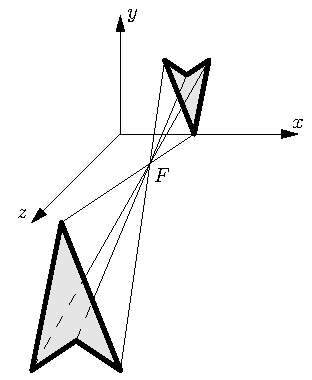
\includegraphics{figures/fig1_8_1.pdf}
    \caption{到$x$-$y$平面上的透视投影：$F$是投影中心（焦点）}
    \label{fig_2}
\end{figure}

这就是照相机的工作原理，也是对我们眼球运作方式的合理且初步的近似。

\begin{figure}[htbp]
    \centering
    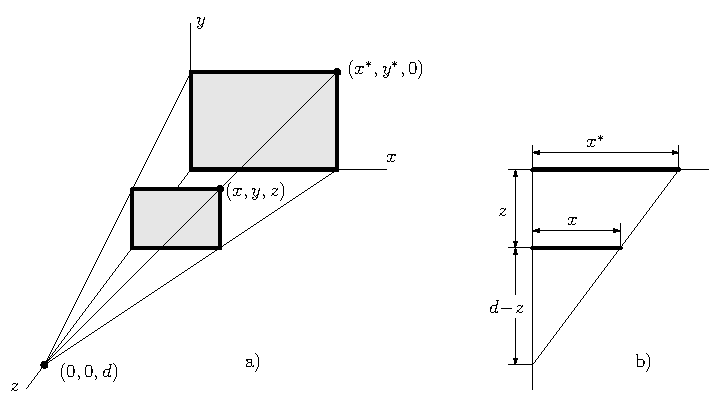
\includegraphics{figures/fig1_8_2.pdf}
    \caption{求出点$(x,y,z)^T$的透视投影的坐标$x^\ast,y^\ast$}
    \label{fig_3}
\end{figure}

下面推导这种投影的公式。假设焦点是$(0,0,d)^T$，并且是向$x$-$y$平面上投影——见图 \ref{fig_3} a)。考虑点$\mathbf{v}=(x,y,z)^T$，并令$\mathbf{v}^*=(x^*,y^*,0)^T$是其投影。如图 \ref{fig_3} b)，分析相似三角形可得\[\frac{x^*}{d}=\frac{x}{d-z},\]
故\[x^*=\frac{xd}{d-z}=\frac{x}{1-z/d},\]
类似有\[y^*=\frac{y}{1-z/d}.\]
注意，此公式同样适用于$z>d$和$z<0$的情况：你可以自行绘制对应的相似三角形来检验。

于是透视投影将点$(x,y,z)^T$映射到点$\begin{pmatrix}\frac{x}{1-z/d},\frac{y}{1-z/d},0\end{pmatrix}^T$。

该变换显然不是线性的（由于分母中的$z$）。然而，可以将它表示为线性变换。为此，我们引入所谓{\bf 齐次坐标}。

在齐次坐标中，$\mathbb{R}^3$中的每个点都用$4$个坐标来表示，其中最后一个（即第$4$个）坐标充当缩放系数的角色。从而，要从向量$\mathbf{v}$的齐次坐标$(x_1,x_2,x_3,x_4)^T$恢复出通常的$3$维坐标$(x,y,z)^T$，我们需要将每项都除以最后一个坐标$x_4$，再取前三个坐标\footnote{如果我们将$\mathbb{R}^3$中一个点的齐次坐标乘以一个非零标量，这个点不会改变。换言之，在齐次坐标中，$\mathbb{R}^3$中的点是用$\mathbb{R}^4$中过$\mathbf{0}$的直线来表示的。}（若$x_4=0$，那么此办法就不奏效了，因此我们假设$x_4=0$对应的是处于无穷远处的点）。

于是在齐次坐标中，向量$\mathbf{v}^{*}$可表示为$(x,y,0,1-z/d)^T$，因此在齐次坐标中，透视投影是线性变换：
\[\begin{pmatrix}x\\y\\0\\1-z/d\end{pmatrix}=\begin{pmatrix}1&0&0&0\\0&1&0&0\\0&0&0&0\\0&0&-1/d&1\end{pmatrix}\begin{pmatrix}x\\y\\z\\1\end{pmatrix}.\]
注意在齐次坐标中，平移也是线性变换：\[\begin{pmatrix}x+a_1\\y+a_2\\z+a_3\\1\end{pmatrix}=\begin{pmatrix}1&0&0&a_1\\0&1&0&a_2\\0&0&1&a_3\\0&0&0&1\end{pmatrix}\begin{pmatrix}x\\y\\z\\1\end{pmatrix}.\]

不过，如果投影中心不是$(0,0,d)^T$，而是任意的点$(d_1,d_2,d_3)^T$呢？那么，我们需要首先做平移量为$-(d_1,d_2,0)^T$的平移，将投影中心移到$(0,0,d_3)^T$（同时保持$x$-$y$平面不变），再作用该投影，然后再用平移量为$(d_1,d_2,0)^T$的平移来抵消之前的平移。类似地，如果投影平面不是$x$-$y$平面，就需要通过旋转和平移将投影平面转到$x$-$y$平面上，之后的逻辑类似上述过程。

所有这些运算都仅仅是与$4\times 4$矩阵的乘法。这就能够解释为何现代的显卡在处理器中内置了$4\times 4$矩阵运算。

当然，此处我们只是对$3$维图形学背后的数学有了粗浅的认识，还有许多可供了解的地方。例如，怎样确定一个物体的哪些部分是可见或不可见的，如何制造逼真的光影，等等。

\begin{problemset}
    \item $\mathbb{R}^3$中的哪个向量具有齐次坐标$(10,20,30,5)$？
    \item 证明：旋转$\gamma$可表示为以下这两个“剪切与缩放”变换的复合：
    \[T_1=\begin{pmatrix}1&0\\\sin\gamma&\cos\gamma\end{pmatrix},\quad T_2=\begin{pmatrix}\sec\gamma&-\tan\gamma\\0&1\end{pmatrix}.\]
    两变换的顺序应该是什么样？
    \item 将$2$维向量乘以任意$2\times 2$矩阵通常需要做$4$次乘法。
    
    假设$2\times 1000$矩阵$D$包含$\mathbb{R}^2$中的$1000$个点。利用两个任意的$2\times 2$矩阵来变换这些点，需要做多少次乘法？请比较两种可能的算法，$A(BD)$和$(AB)D$。
    \item 写出表征投影中心为$(d_1,d_2,d_3)^T$、投影平面为$x$-$y$平面的透视投影的矩阵。
    \item $\mathbb{R}^3$中的变换$T$将向量绕$x$-$y$平面中的直线$y=x+3$旋转$\gamma$。写出对应于该变换的$4\times 4$矩阵。
    
    你可将答案保留为若干矩阵相乘的形式。
\end{problemset}